\documentclass[../main.tex]{subfiles}
\graphicspath{{\subfix{./figs/}}}
%\addbibresource{../ut_thesis.bib}

% to do:
%    - cross sections explanation
%    - strangeness production explanation
%    - factorization
% images
%     - cosmological 
%     - asymptotic freedom
%     - QCD phase diagram
%     - heavy ion collision
%     - jets
%     - quenching
%     - mandelstam invariants (S)
%     - hadronization
%     - Bjorken x, Q2
%     - curves of constant proper time
%     - basic overview of TPC, ITS, TOF, EMCal, HCal
\begin{document}

\section{A Crash Course in Particle Physics}

\subsection{The Standard Model}
Given our current understanding of the universe, there are four fundamental forces governing the interactions between all known particles: 

\begin{itemize}
    \item Strong Force: The strongest interaction, describing the dynamics of quarks and gluons. This interaction is described by quantum chromodynamics. The strong force is relevant on length scales within a proton or neutron. 
    \item Electromagnetism: Responsible for electricity and magnetism, describing photons and particles that carry electric charge. 
    \item Weak Force: Responsible for nuclear decays. This is the only interaction that can change flavor. The weak force is also the only interaction that is not symmetric under parity. 
    \item Gravity: Describes the gravitational force, relevant from human to cosmological scales in spacetime. 
\end{itemize}

The \textit{Standard Model} describes the strong force, electromagnetism, and the weak force. This is the arena of particle and nuclear physics. Our best description of gravity comes from \textit{general relativity}, which describes spacetime on the largest scales by endowing it with a metric field. Since the effects of gravity are only measurable on large scales, it is not relevant at the small scales probed at our current colliders, and will not be expanded upon in this thesis. 

The underlying framework behind the Standard Model is quantum field theory. In a hand-wavy sense, to each type of particle we associate a field; particles are excitations in these fields (ie. an electron is an excitation in the electron field). Whether two given fields are coupled determines whether they can interact. The Standard Model is an effective field theory, so we can write down a Lagrangian density for it, from which, in principle, we can derive the dynamics for a given system. In practice, this is extremely difficult.   

One way of conceptualizing particle interactions via the Standard Model is through the exchange of gauge bosons. For example, the photon mediates electromagnetism, while the gluon mediates the strong force. Whether a particle feels a force depends on if it carries the charge of the force. Quarks are the only fundamental particles that participate in the strong interaction because they carry \textit{color charge}, while all other massive particles---the leptons---do not carry this charge. A basic diagram of the Standard Model particles is shown in Fig. \ref{fig:standard_model}.

\begin{figure}[h]
    \centering
    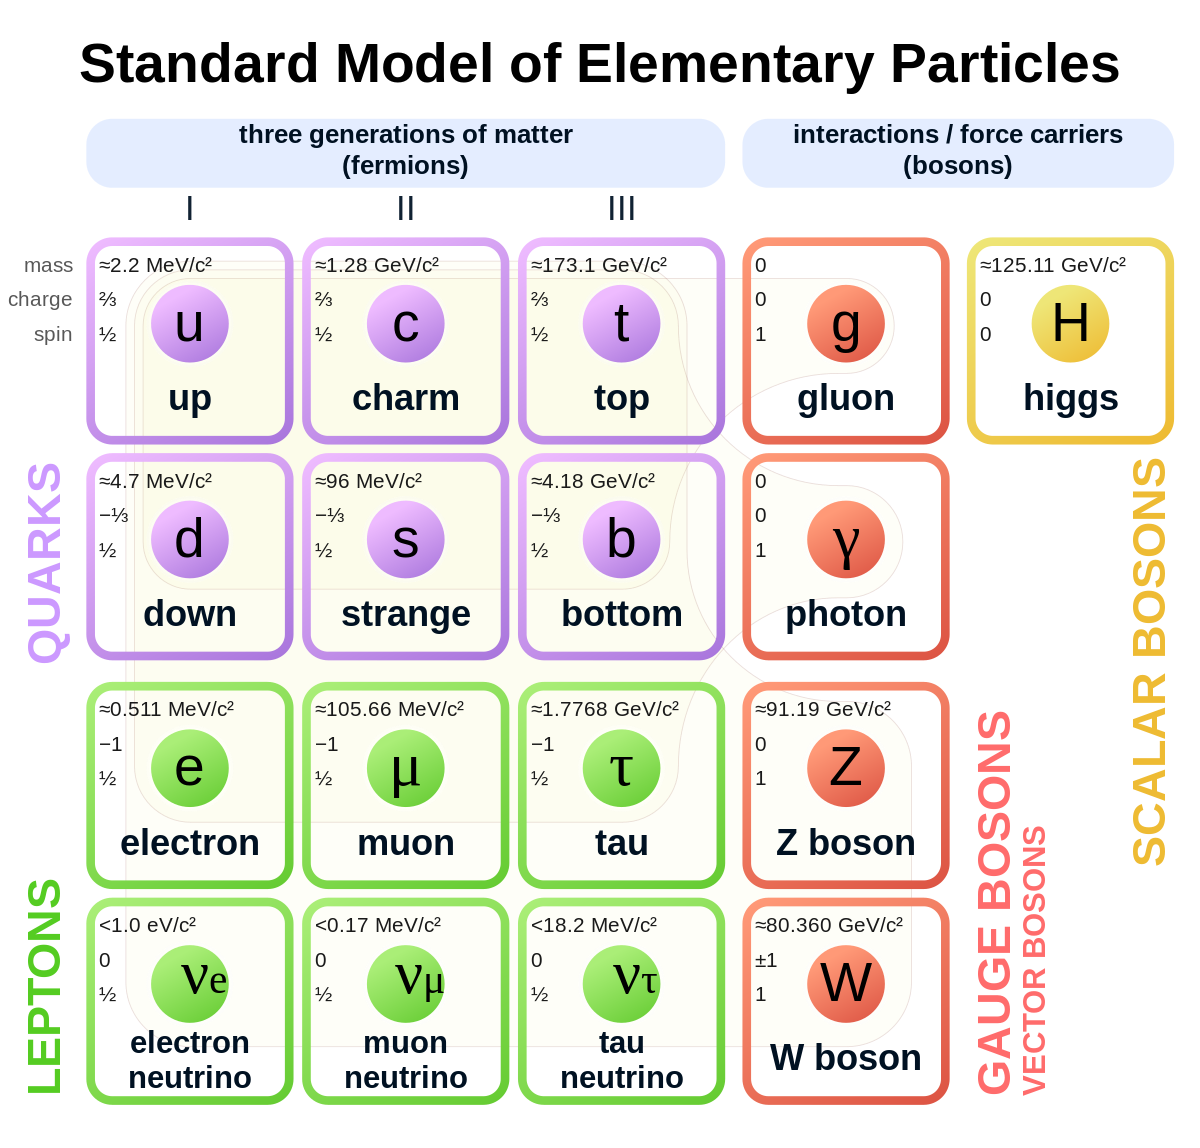
\includegraphics[scale=0.2]{introduction/figs/standardmodel.png}
    \caption{The Standard Model of particle physics. From: \textit{Wikipedia}.}
    \label{fig:standard_model}
\end{figure}


\subsection{Quantum Chromodynamics}
Quantum chromodynamics (QCD), also known as the strong force or color force, describes the dynamics between quarks and gluons. The name comes from the fact that there are three types of charge, known as color charge: red, green, and blue. This theory is incredibly complicated because unlike with photons and electromagnetism, the carriers of the strong force---the gluons---carry the charge of the interaction. There are eight types of gluon, corresponding to different color states. This makes calculations in QCD particularly challenging. In addition, there are two unusual features of QCD, known as asymptotic freedom and color confinement. 

\begin{figure}[h]
    \centering
    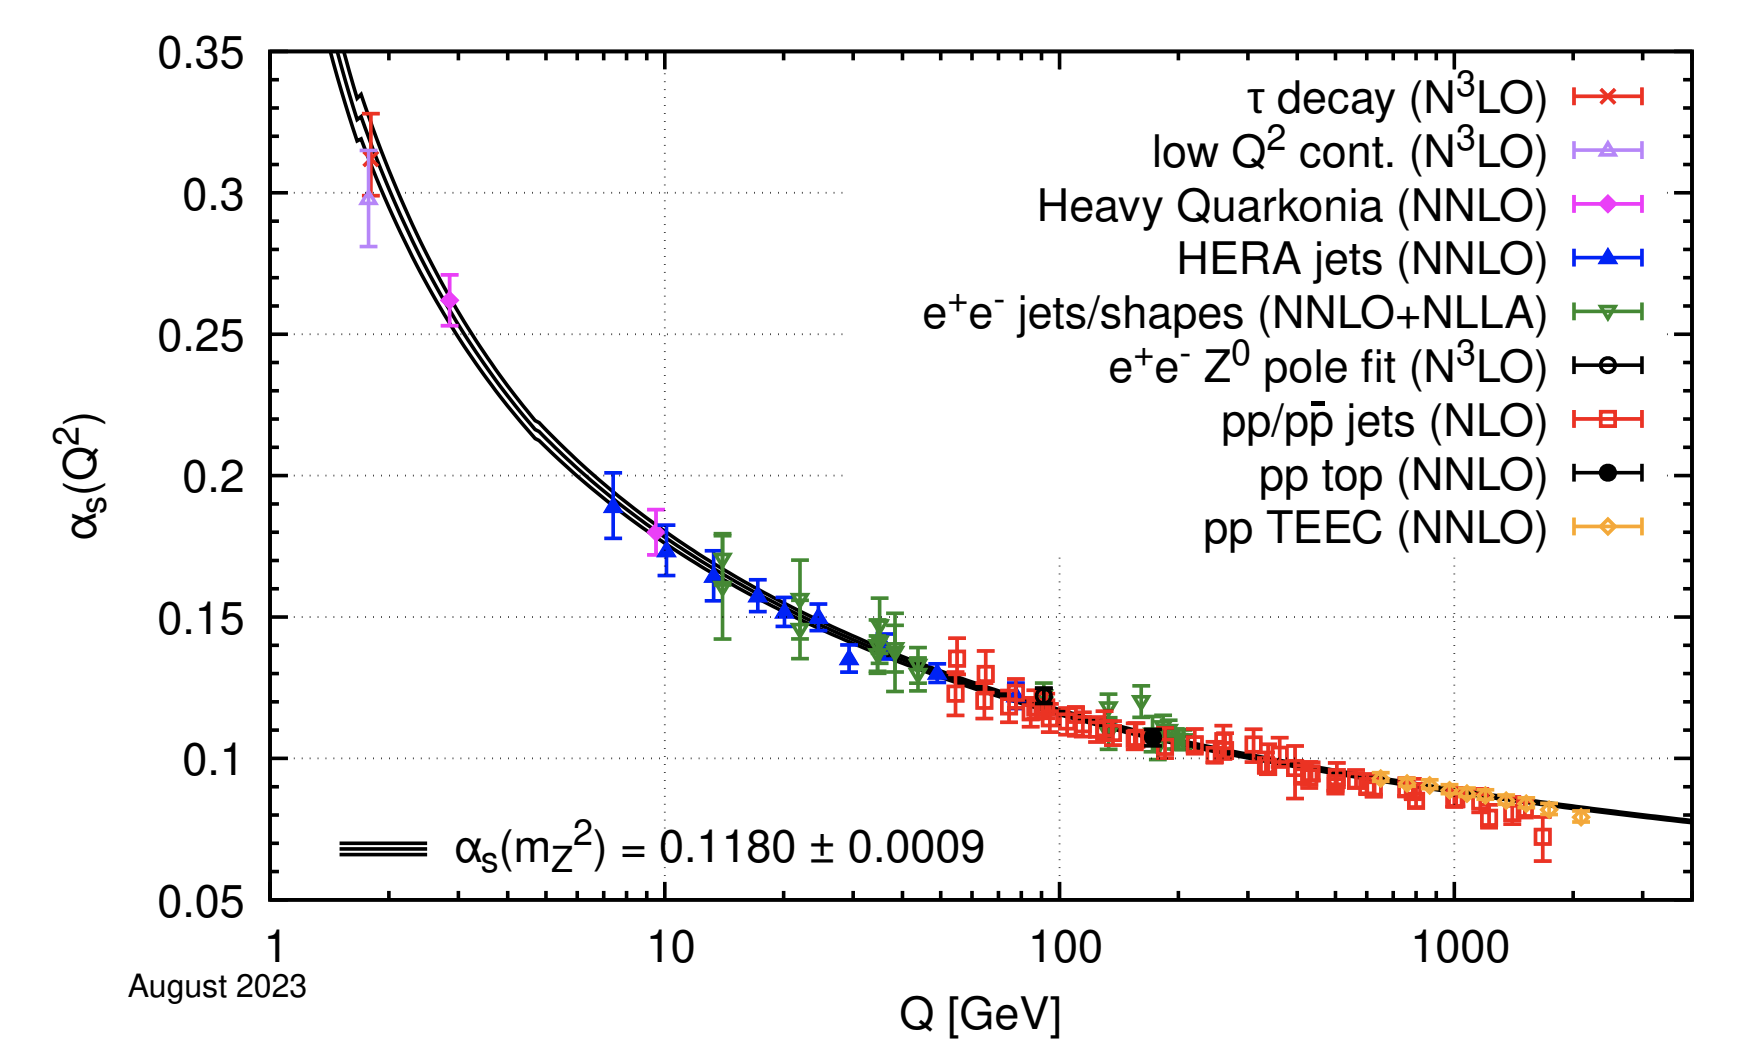
\includegraphics[scale=0.2]{introduction/figs/asymptotic.png}
    \caption{A plot of $\alpha_s$ across various energy scales. As the energy scale increases, the coupling constant decreases asymptotically \cite{Workman:2022ynf}.}
    \label{fig:asymptotic}
\end{figure}

In quantum field theory, a common method to make headway on a problem is to utilize perturbation theory. This is only possible if the coupling constant associated with the interaction is less than one, however this is often not true in the case of the strong force. This makes understanding QCD extremely difficult. However, as the energy scale of the problem increases (or the length scale decreases), the value of the strong coupling constant $\alpha_s$ decreases (Fig. \ref{fig:asymptotic}). We call this phenomenon asymptotic freedom, for which the $2004$ Nobel Prize in Physics was awarded to David Gross, Frank Wilczek, and David Politzer. In this regime, we can utilize perturbative QCD (pQCD) to solve problems. 

If we take a $q$-$\bar{q}$ bound state and try to separate the pair, we have to put so much energy in that we simply create two new $q$-$\bar{q}$ pairs. The important consequence is that we will never observe a lone quark. We can model this potential as a linear one for large separations:

\begin{equation} 
    \label{eq:cornell}
    V(r) = \frac{-4}{3}\frac{\alpha_s}{r} + \sigma r + c 
\end{equation}

where $r$ is the separtion between the quarks, $\sigma$ is a constant that acts like a string tension, and $c$ is a constant. This effective model of color confinement is expanded on in Section \ref{sxn:pythia}. 

\begin{figure}[h]
    \centering
    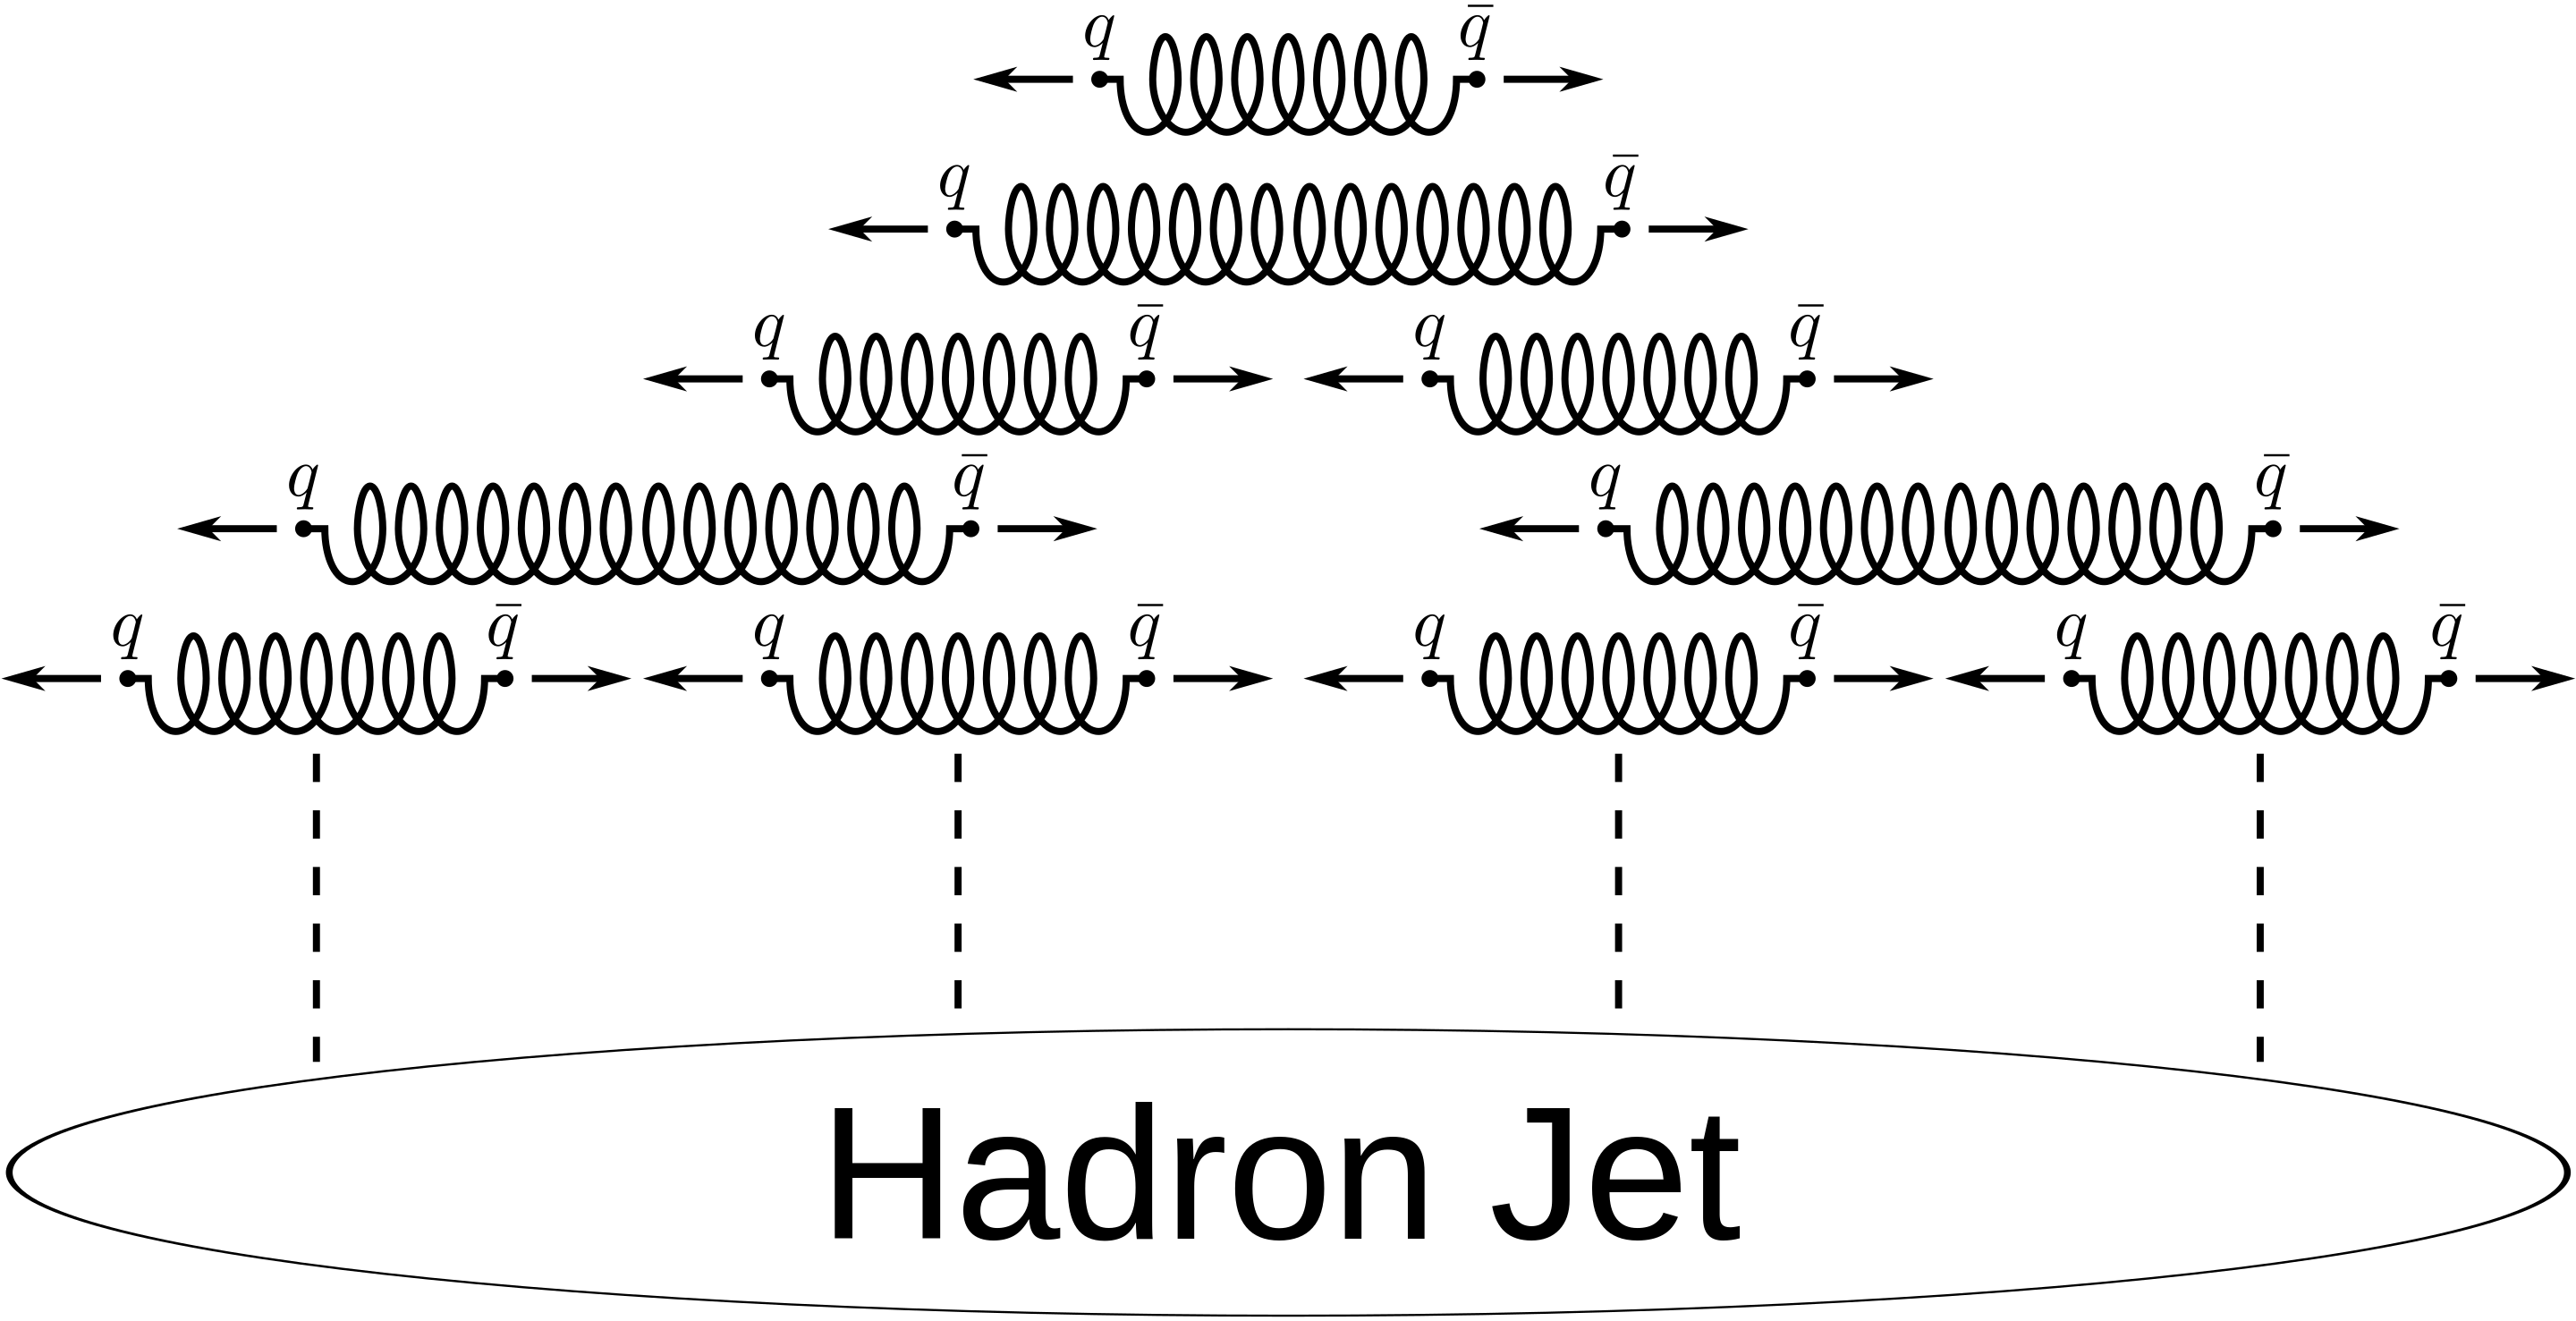
\includegraphics[scale=0.1]{introduction/figs/confinement.png}
    \caption{A depiction of how a \text{jet} is formed. In collider physics, scatterings between partons that involve high momentum transfer can produce two outgoing high-momentum partons. In this example, a $q$-$\bar{q}$ pair is produced. As the original $q$-$\bar{q}$ pair separates, new pairs are formed. This is due to color confinement.}
    \label{fig:confinement}
\end{figure}



\subsection{Hadrons! Hadrons! Hadrons!}
Due to color confinement, we will never observe lone partons (quarks and gluons). Instead, we only see color-neutral bound states called \textit{hadrons}. For a meson, a hadron consisting of two quarks, this can be accomplished by having a quark and anti-quark with opposite color charge. For a baryon, consisting of three quarks\footnote{Technically, a meson consists of an even number of quarks and a baryon consists of an odd number. In reality, a meson with more than $2$ quarks and a baryon with more than $3$ are extremely rare.}, we would have a red, green, and blue quark (or anti-red, anti-green, and anti-red) which adds up to white (color-neutral). Note, when we count quarks in hadrons, we are referring to the valence quarks which is a simplification. Hadrons like the proton are actually extremely dynamic, with $q$-$\bar{q}$ pairs popping in-and-out of existence while gluons whiz about---this is known as the quark sea. 

\begin{figure}[h]
    \centering
    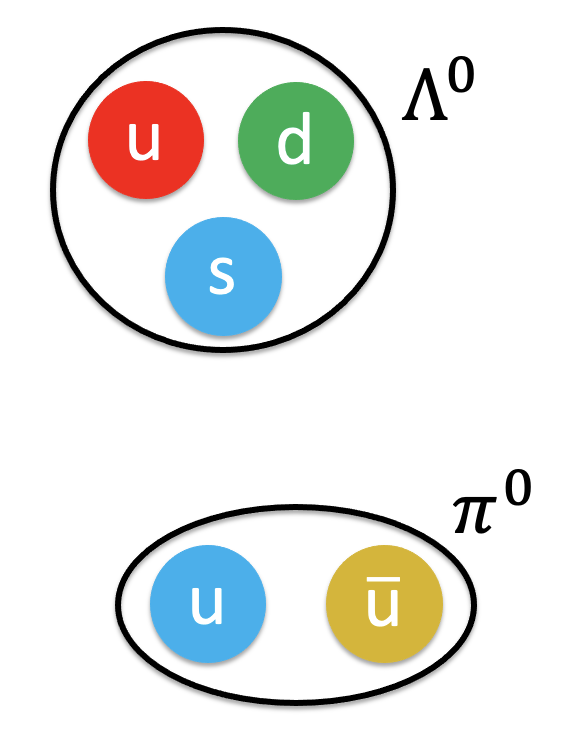
\includegraphics[scale=0.2]{introduction/figs/hadrons.png}
    \caption{An example of two hadrons. Importantly, the color charge adds to color-neutral in each case. The $\Lambda^0$ is relevant to this analysis.}
    \label{fig:enter-label}
\end{figure}

The lifetime of a hadron is related to the interaction that mediates its decay, as demonstrated in Fig. \ref{fig:lifetimes}. Strong decays lead to the shortest lifetimes ($\sim$ fm/c). At hadron colliders, we only detect the final-state hadrons that reach our detector. 
To study the underyling partonic dynamics, we must work up the chain, reconstructing decays from the final-state particles. Remarkably, the proton is the only stable hadron, with a lifetime constrained above $10^{34}$ years (the universe is $13\times10^9$ years old). If we measure proton decay, this could indicate a possible grand unified theory. 

\begin{figure}[h]
    \centering
    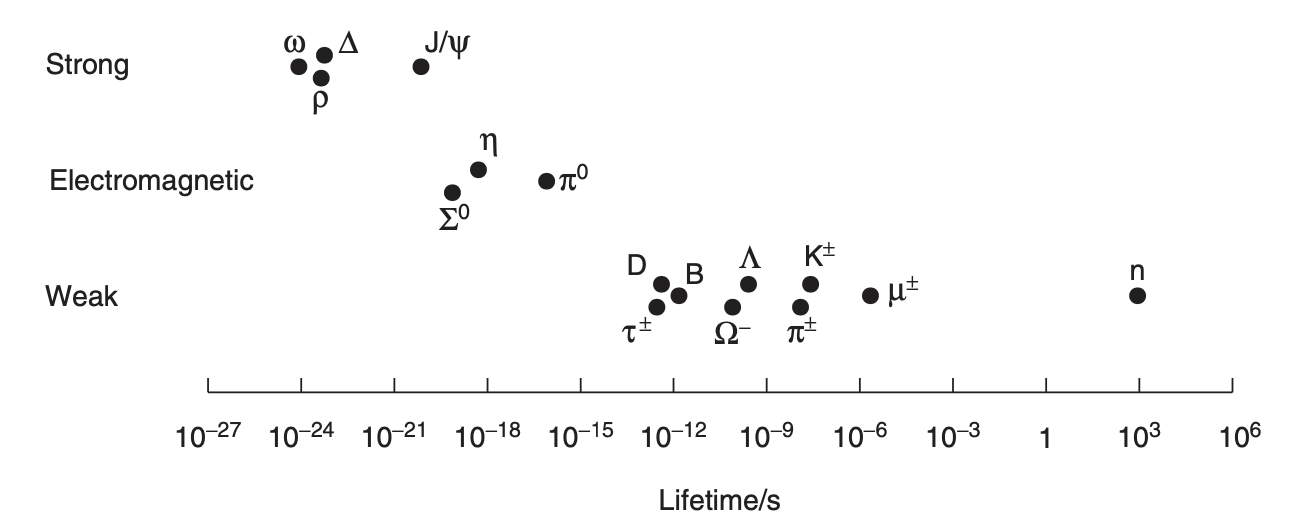
\includegraphics[scale=0.3]{introduction/figs/lifetimes.png}
    \caption{A rough plot of hadrons arranged by their lifetime and type of decay \cite{Thomson:particle}.}
    \label{fig:lifetimes}
\end{figure}

\subsection{Relativistic Kinematics}
At the Large Hadron Collider, particles are accelerated to nearly the speed of light before they collide. This is solidly in the regime of special relativity, where time and space blend into a unified spacetime. Typically, we define a right-handed coordinate system with $z$ along the beamline, as shown in Fig. \ref{fig:alice_coords}. 

\begin{figure}[h]
    \centering
    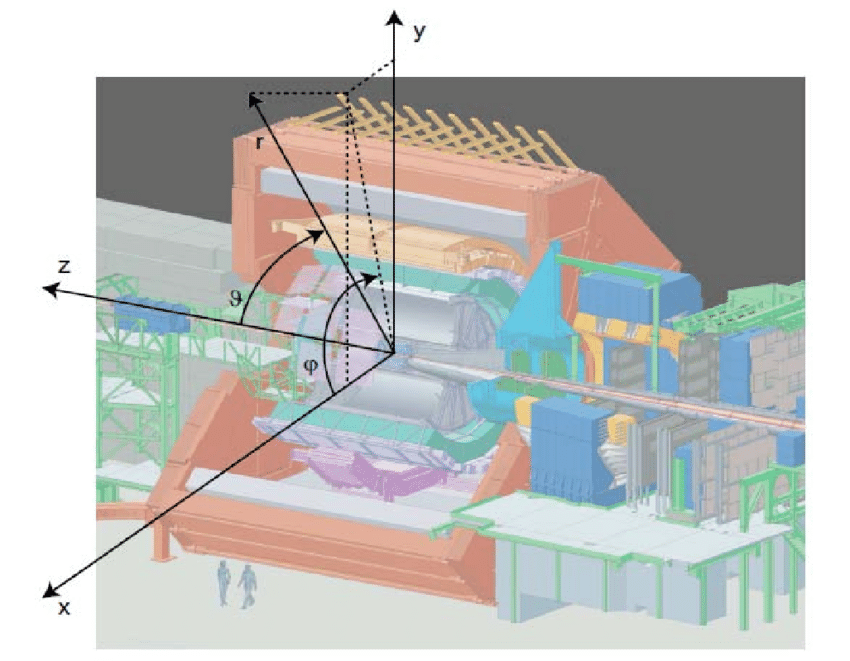
\includegraphics[scale=0.3]{introduction/figs/alice_coords.png}
    \caption{The ALICE coordinate system is a right-handed coordinate system with $z$ aligned along the beam. The transverse plane, or the $x$---$y$ plane, is perpendicular to the $z$-axis. The longitudinal direction and $z$-axis are synonymous.}
    \label{fig:alice_coords}
\end{figure}

Denote the lab frame as the unbarred frame. Let us consider an inertial frame that moves with velocity $v_z$ in the $z$ direction, representing a particle whose rest frame we denote as the barred frame. We can transform four-vectors from the lab frame to the particle's frame using the Lorentz transformation: 

\begin{equation}
    x^{\bar{\mu}} = \sum_{\nu=0}^3 \Lambda^{\bar{\mu}}{}_{\nu} x^{\nu}
\end{equation}

where $\bar{\mu}$ runs from $0$ to $3$. Explicitly, the Lorentz transformation can be written as a matrix:

\begin{equation}
    \Lambda^{\bar{\mu}}{}_{\nu} =  \begin{pmatrix} \cosh{y} & 0 & 0 & -\sinh{y} \\ 0 & 1 & 0 & 0 \\ 0 & 0 & 1 & 0 \\ -\sinh{y} & 0 & 0 & \cosh{y} \end{pmatrix}
\end{equation}

where $y=\tanh^{-1}{v}$ is the boost parameter, also known as the rapidity. Since we are boosting into a frame that moves with $v_z$ along the z-axis:

\begin{align}
    y = \tanh^{-1} v_z & = \tanh^{-1} \frac{\gamma m v_z}{\gamma m} \\
    & = \tanh^{-1} \frac{p_z}{E} \\
    & = \frac{1}{2} \ln{\frac{1 + \frac{p_z}{E}}{1 - \frac{p_z}{E}}} \\
    & = \frac{1}{2} \ln{\frac{E + p_z}{E - p_z}}
\end{align}

This is the familiar expression for rapidity used in collider physics. For a high momentum particle with most of its momentum in the $x$---$y$ plane, $p_z \approx 0$ so $y \approx 0$. For a high momentum particle with most of its momentum in the $z$ direction, $E \approx p_z$ and, in the limit, $y \rightarrow \infty$. Similarly, if most of the momentum is in the $-z$ direction, then $y \rightarrow - \infty$. Thus, for relativistic particles, rapidity is related to the angle of emission from the beam axis. We use rapidity instead of $\theta$ because differences in rapidity are Lorentz invariant. Thus, when boosting between the lab frame and center-of-mass frame, $y$ distributions are merely shifted, not distorted. 

To see this fact, consider three inertial frame $A$, $B$, and $C$. To boost from $A$ to $C$, we could boost from $A$ to $B$ and then from $B$ to $C$. This is equivalent to simply adding the rapidities when used as the boost parameter:

\begin{equation}
    \Lambda({y_{AC}}) = \Lambda (y_{AB}) \Lambda(y_{BC}) = \Lambda(y_{AB} + y_{BC})  
\end{equation}

Thus, 

\begin{equation}
    y_{AC} = y_{AB} + y_{BC}  
\end{equation}

Since rapidity is related to the angle of emission of a relativistic particle from the beam line, it is conventient to define pseudorapidity, $\eta$: 

\begin{equation}
    \eta \equiv \frac{1}{2} \ln{\frac{|\mathbf{p}| + p_z}{|\mathbf{p}| - p_z}} = - \ln{ \left[  \tan{\left( \frac{\theta}{2}  \right)} \right]}
\end{equation}

Pseudorapidity can be explicity written in terms of the angle from the beam axis, and for relativistic particles $m \ll |\mathbf{p}| \implies E \approx p$, so $y \approx \eta$. Since pseudorapidity is directly related to the angle of emission and differences in pseuodrapidity are approximately Lorentz invariant, we use $\eta$ instead of rapidity. We refer to $\eta$ values near $0$ as midrapidity and values far from $0$ as forward rapidities. 

\begin{figure}[h]
    \centering
    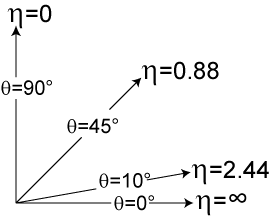
\includegraphics[scale=0.5]{introduction/figs/pseudorapid.png}
    \caption{A diagram demonstrating how pseudorapidity relates to $\theta$, the angle from the beamline. Source: \textit{Wikipedia}.}
    \label{fig:pseudorapid}
\end{figure}


\subsection{Cross Sections}
Scattering is the heart of experimental particle physics. If we want to know the structure of some substance, we can scatter particles off of it, see what comes out, and reconstruct what happened. This is how the famed Rutherford gold foil experiment determined atomic nuclei exist. This is also how deep inelastic scattering demonstrated there are three point-like particles---valence quarks---in the proton. 
Even in other areas of physics, scattering experiments are ubiquitous. For example, electron microscopes scatter a beam of electrons off a target to resolve an image.\footnote{In a sense, this makes Electron-Ion Collider the world's soon-to-be largest electron microscope.} If we are being slightly facetious, then we can even say a microscope scatters light off a target, recollecting that scattered light into your eye to make an image. 

To quantitatively understand scattering, let's consider a fixed-target experiment, where we shoot a beam of particle species $1$ at a stationary target consisting of particle species $2$. We can characterize this experiment by how often an interaction happens. The higher the flux of the incident beam, the higher the rate of interaction per particle species $2$. We can thus write:

\begin{equation}
    R_2 = \sigma \phi_1
\end{equation}

where $\sigma$ is the \textit{cross section}, a constant of proportionality with dimensions of area. We can conceptualize $\sigma$ as the effective area of each target particle, but this is rarely actually true. The cross section characterizes the probability of a given interaction, abstracting away the underlying quantum mechanics. 

In experiments like deep inelastic scattering or the Rutherford experiment, a beam of particles is scattered off of a target, and the angular distribution of the scattered particles gives information about the structure of the target. To capture this angular information, it's useful to work with the differential cross section $d\sigma/d\Omega$, where:

\begin{equation}
    \sigma = \int \frac{d\sigma}{d\Omega} d\Omega
\end{equation}

In short, the differential cross section is the rate per target particle of incident particles scattered into a certain solid angle, divided by the incident flux. This cross section is a function of both $\theta$ and $\varphi$, but often symmetry in $\varphi$ allows us to reduce the differential cross section to a function of just $\theta$. 

\begin{figure}[h]
    \centering
    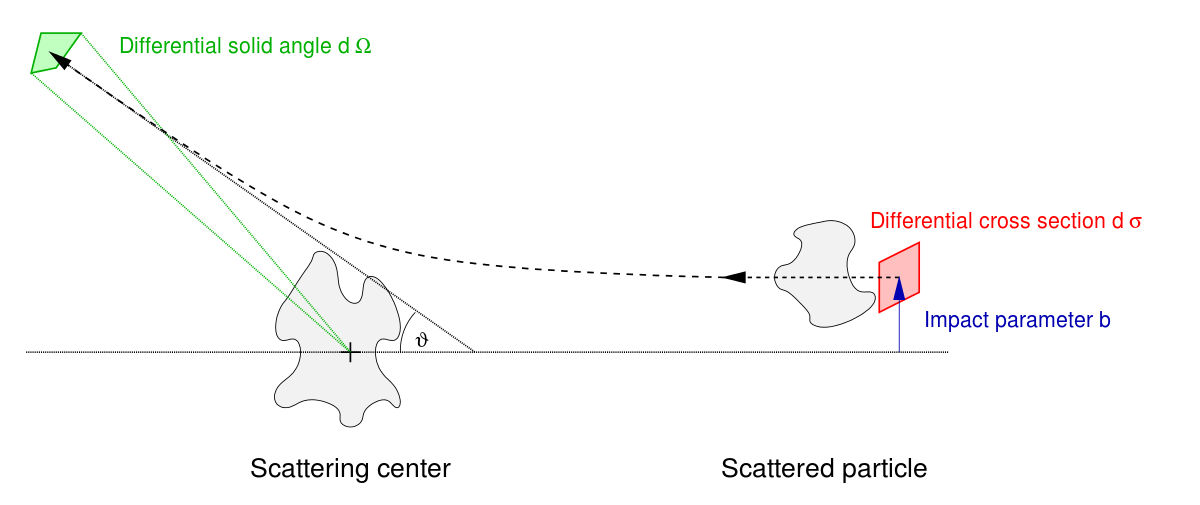
\includegraphics[scale=0.35]{introduction/figs/diffcross.png}
    \caption{The set-up of a standard scattering problem. A particle originally parallel to the $z$-axis scatters off a target, leaving at an angle $\vartheta$. This angle is called the scattering angle. The differential cross section gives the probability a particle passing through an area $d\sigma$ is scattered into some solid angle $d\Omega$. Source: \textit{Wikipedia}.}
    \label{fig:enter-label}
\end{figure}

As an example of a differential cross section, let us consider scattering in a Coulomb potential---the \textit{only} potential where the cross section obtained from quantum and classical calculations agree. Let $Z_1e$ be the charge a particle incident on a second particle of charge $Z_2e$, where $e$ is the elementary charge. If the incident particle has initial velocity $v_0$, this differential cross section, also known as the Rutherford cross section, is then given by: 

\begin{equation}
    \frac{d\sigma}{d\Omega}(\vartheta) = \left(\frac{Z_1 Z_2 e^2}{8 \pi \epsilon_0 m v_0^2}\right)^2 \csc^4{(\vartheta / 2)}
\end{equation}

This represents the angular distribution of scattered particles. Philosophically, the differential cross section tells us how the final state distribution of particles relates to the initial state. Often, the initial state represents particles fired along the $z$-axis, and the final state is the angular distribution of scattered particles. However, differential cross sections are not restricted to angular distributions. One can also define cross sections in terms of $E$ or other kinematic variables:

\begin{equation}
    \frac{d\sigma}{dE}    
\end{equation}

or define two-dimensional differential cross sections:

\begin{equation}
    \frac{d^2\sigma}{dE d\eta}
\end{equation}

% https://physics.stackexchange.com/questions/438335/theoretical-definition-and-pratical-mesurement-of-differential-cross-section
\subsection{Feynman Diagrams}
Feynman diagrams are an important calculational tool in particle physics, representing the transition between two quantum states. In fact, these pictorial representations actually allow us to work out the probability of a given interaction. Consider the diagram in Fig. \ref{fig:twotwo}, representing the $2\rightarrow2$ process $a$ + $b$ $\rightarrow$ $c$ + $d$. By this notation, we mean we start in a state consisting of particles $a$ and $b$, ending in a state consisting of particles $c$ and $d$. The leftmost diagram depicts how the initial and final states are related by the exchange of the boson $X$. This diagram actually represents two possible time-orderings of the process, which becomes relevant when we need to actually calculate interaction probabilities. From quantum field theory, we can cook up rules for calculating from these diagrams, and a given process generally has an infinite number of associated diagrams. If the coupling constant for a given interaction is small (eg. electromagnetism where $\alpha \approx 1/137$) then we need only consider the highest order diagrams. Unfortunately, in the case of QCD where $\alpha_s \approx 1$ unless we are at high energy scales, this makes calculations intractable. In a sense, collider experiments measure final state particles to reconstruct the original process represented by these Feynman diagrams.  

\begin{figure}[h]
    \centering
    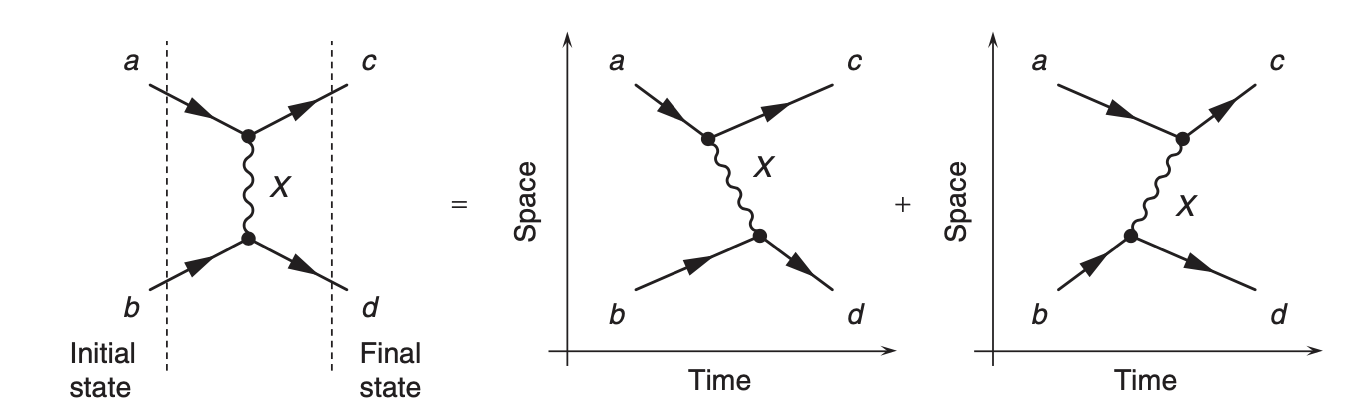
\includegraphics[scale=0.3]{introduction/figs/twotwo.png}
    \caption{A depiction of Feynman diagrams for the general process $a$ + $b$ $\rightarrow$ $c$ + $d$, mediated by a gauge boson $X$. The leftmost diagram that summarizes the interaction actually represents two possible time-orderings \cite{Thomson:particle}.}
    \label{fig:twotwo}
\end{figure}


\subsection{Understanding Hadronization and Jets}

Due to color confinement, we will never observe a lone quark. At some point, the partons in a given high energy interaction must undergo hadronization, the formation of color-neutral bound states. Since hadronization is non-perturbative, we must resort to models to understand the process. Let's examine a common model of hadronization---the \textit{Lund string model}---in the context of the simple $2 \rightarrow 2$ process $e^+e^- \rightarrow q\bar{q}$, with the associated Feynman diagram shown in Fig. \ref{fig:elecpos}. In the Lund string model, the two quarks produced in the interaction are initially free and move apart with high relative velocity. A color flux tube, also called a string, connects the two quarks, representing energy in the color field between the pair. The force across the tube is assumed constant, like tension in a string, which gives rise to a linear potential in the separation (Eq. \ref{eq:cornell}). As the quarks separate, energy is transferred from the partons to the color flux tube until it is energetically favorable for the tube to snap and two pairs of quarks connected by smaller tubes form. We can imagine this like stretching an elastic string until it reaches the yield point and breaks. The smaller strings that connect the two new pairs of partons continue to fragment further and further, producing two clusters of hadrons that each move in the direction of the original quarks. Each cluster of hadrons is called a jet, which we measure in a detector. A cartoon of this process is depicted in Fig. \ref{fig:confinement}. Thus, jets of hadrons give us information about the underlying partonic processes.

\begin{figure}[h]
    \centering
    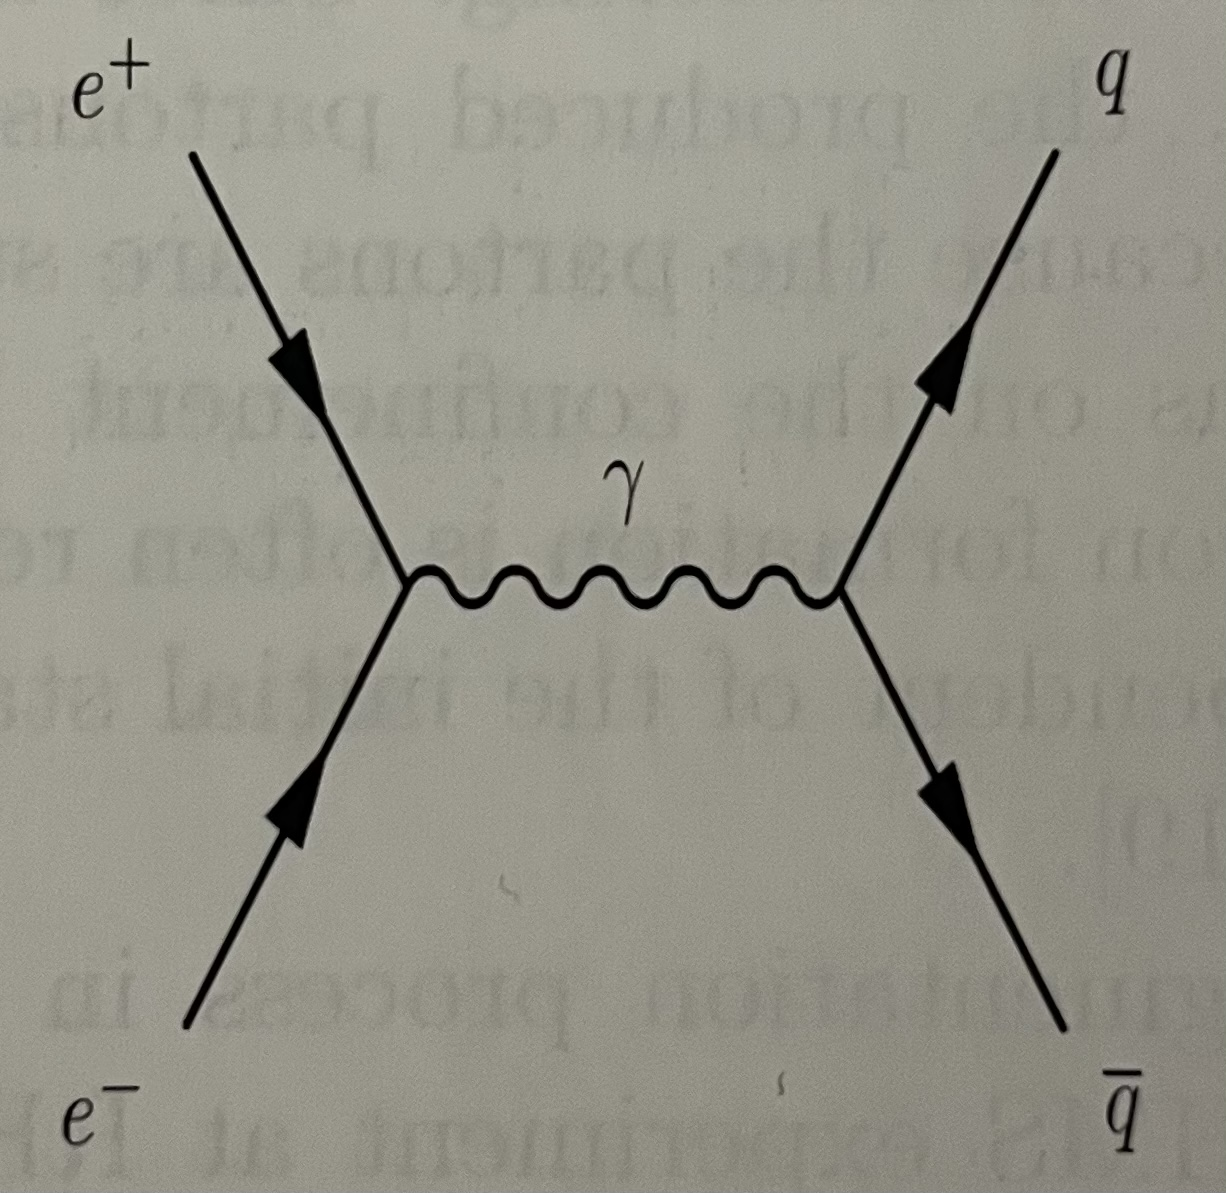
\includegraphics[scale=0.5]{introduction/figs/elecpos.jpeg}
    \caption{A simple Feynman diagram describing $e^+e^- \rightarrow q\bar{q}$, taken from \cite{Vogt:2007zz}.}
    \label{fig:elecpos}
\end{figure}

To quantify how hadrons are produced from partonic scattering, we utilize \textit{fragmentation functions}. Consider the $2 \rightarrow 2$ scattering $e^+e^- \rightarrow q \bar{q}$. The quark fragments into a hadron $h$ which is observed in the detector. If we denote the center-of-mass energy as $Q$, then in the center-of-mass frame each beam has energy $Q/2$. Due to momentum conservation, the quark and anti-quark are produced in opposite directions, and each carry energy $Q/2$. We can thus define $z$, the energy the final-state hadron carries $E_h$ over the fraction of energy the quark initially had:

\begin{equation}
    z = \frac{2 E_h}{Q}
\end{equation}

Which allows us to define a differential cross-section as a function of $z$ \cite{Vogt:2007zz}:

\begin{equation}
    \frac{d\sigma{(e^+e^- \rightarrow hX})}{dz} = \sum_q \sigma(e^+e^- \rightarrow q\bar{q})[D_q^h(z) + D_{\bar{q}}^h(z)]
\end{equation}

where $q$ is a sum over quark flavors and $\sigma$ is a cross section related to the underlying partonic process. Here $D_q^h$ is the fragmentation function which represents the probability of producing a final-state hadron with momentum fraction $z$. Importantly, fragmentation functions are assumed universal---intrinisic to a certain process. Thus, fragmentation functions measured from $e^+e^-$ collisions should also apply to $pp$ collisions. This example is analogous to the initial hard scatterings in a heavy-ion collision where two back-to-back partons are produced which hadronize into a dijet (two back-to-back jets). 

Fragmentation functions are reminiscent of \textit{parton distribution functions} which give the probability of observing a quark within a hadron as a function of the momentum fraction of the quark. At hadron colliders, a description of hadronization is much more difficult. To accurately calculate cross-sections, we need to consider higher order diagrams and utilize parton distribution functions. In order to make progress, we rely on factorization theorems which separate partonic cross sections (calculable in pQCD), fragmentation functions, and parton distribution functions. 

%https://arxiv.org/pdf/1607.02521.pdf

\section{The Quark-Gluon Plasma}
The overarching goal of heavy-ion physics is to elucidate the properties of the quark-gluon plasma (QGP), a state of matter that existed in the first microseconds after the Big Bang (Fig. \ref{fig:cosmo}). This represents one patch on the QCD phase diagram (Fig. \ref{fig:phase_diagram}), which maps states of QCD matter for various temperatures and baryon chemical potentials (loosely, density). In this state, the quarks and gluons that are ordinarily locked inside hadrons are deconfined. Thus, by probing the QGP, we can begin to understand the partonic degrees of freedom in QCD while assembling a picture of the early universe. This earns the QGP its nickname as the "primordial soup."

In high energy heavy-ion collisions at the Large Hadron Collider, we produce the necessary conditions to deconfine the quarks and gluons that make up nucleons, leading to the creation of mini QGPs. By studying the final state particles our detectors measure, we can infer the dynamics of these high energy collisions and the QGP. Interestingly, the QGP is a strongly interacting liquid with a tiny shear viscocity to entropy ratio that pushes the limit of what physicists believe is possible \cite{Busza:2018rrf}. This makes the QGP the most perfect liquid ever created. Another unexpected discovery was that the transition from quark-gluon plasma to hadron gas is smooth, rather than a discontinuous cross-over. The critical temperature of the QGP is typically taken as $T_c \approx 160$ MeV (around $10^5$ times hotter than the center of the Sun).

\begin{figure}[h!]
    \centering
    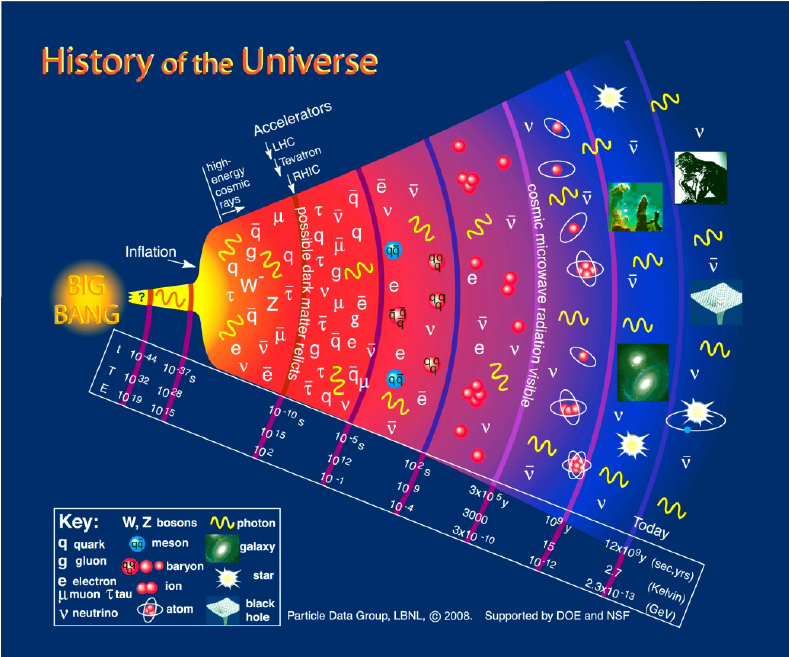
\includegraphics[scale=0.34]{introduction/figs/cosmology.png}
    \caption{A diagram of the history of the universe, from the perspective of a particle physicist. The outline of the diagram roughly corresponds to the scale factor which quantifies the expansion of the universe. Source: Particle Data Group.}
    \label{fig:cosmo}
\end{figure}

\begin{figure}[h!]
    \centering
    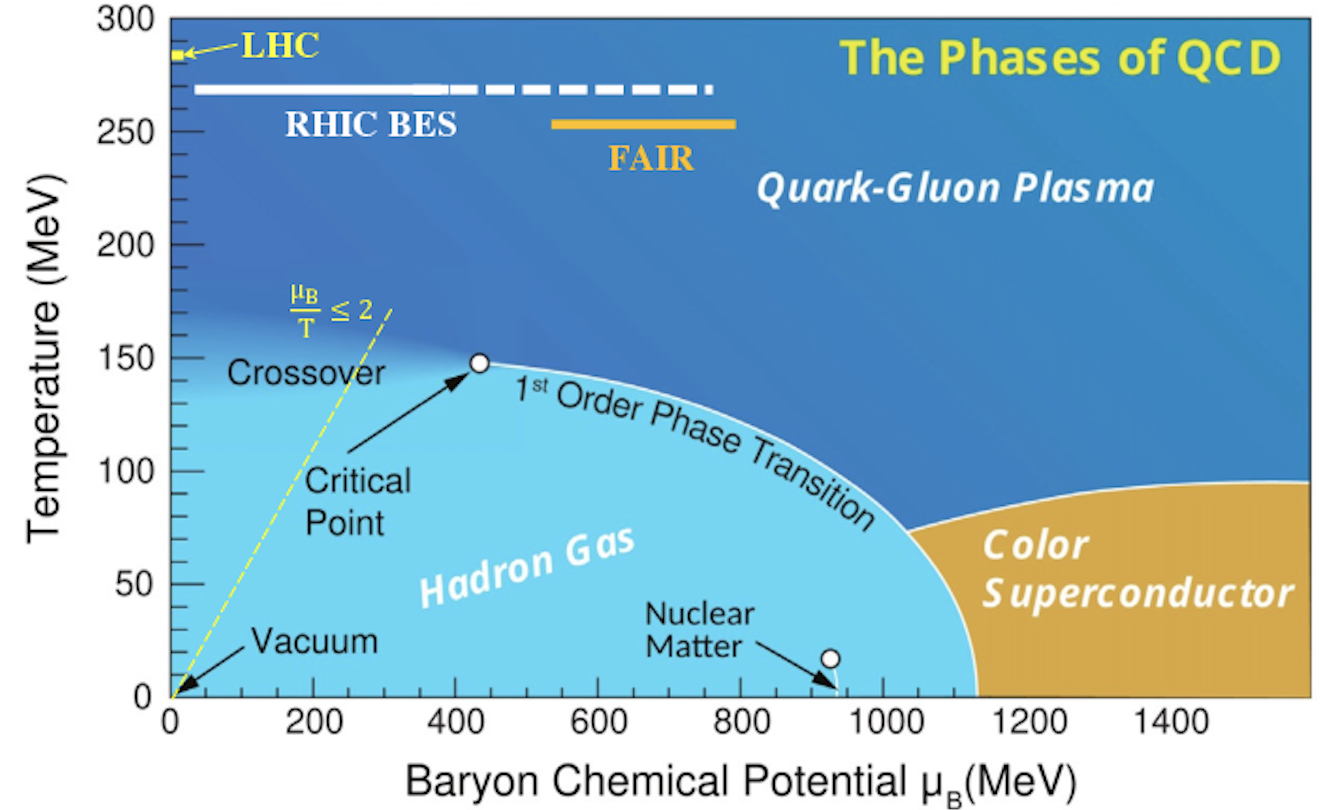
\includegraphics[scale=0.24]{introduction/figs/phasediagram.png}
    \caption{A basic depiction of the QCD phase diagram, the main object of study in relativistic heavy-ion physics \cite{Aprahamian:2015qub}. This diagram is rich unexplored territory and physics.}
    \label{fig:phase_diagram}
\end{figure}

\section{The Anatomy of a Heavy-Ion Collision}
The spacetime structure of a heavy-ion collision is presented in Fig. \ref{fig:spacetime}. The hyperbolae represent lines of constant proper time, an inherent part of Minkowski space. In a relativistic heavy-ion collision, two Lorentz contracted nuclei smack into each other. During the initial stages, certain partons may \textit{hard scatter}, an interaction characterized by large four-momentum exchange. This hard scatter produces jets of hadrons that can reach our detector. After some time, a QGP droplet forms and undergoes hydrodynamic expansion. Next, hadronization begins as the deconfined partons form hadrons. Eventually, inelastic collisions cease and particle abundances are frozen (chemical freeze-out), and elastic scattering ceases, freezing momentum distributions (kinetic freeze-out). The final-state particles then free-stream into the detector where they are measured. The time it takes from the initial hard-scatterings to freeze-out is on the order of $10$ fm/c or $10^{-22}$ s. 

\begin{figure}[h]
    \centering
    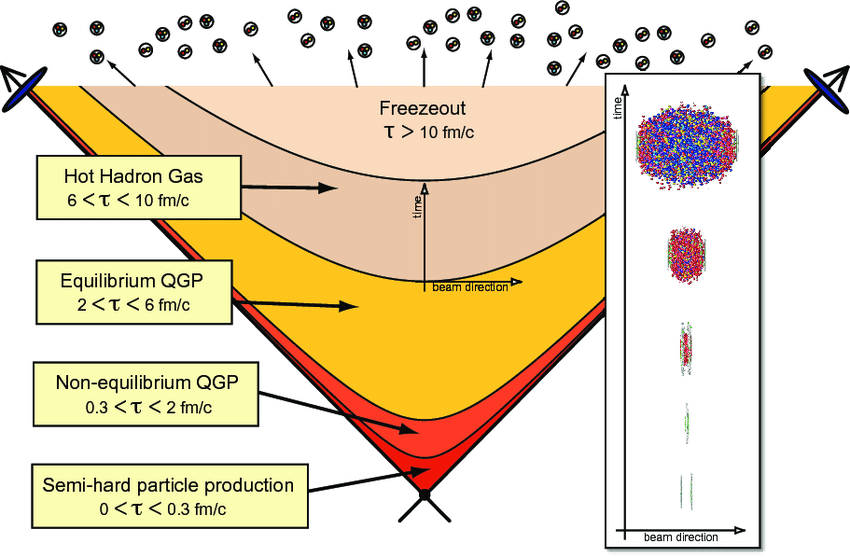
\includegraphics[scale=0.3]{introduction/figs/spacetime.png}
    \caption{The spacetime structure of a heavy-ion collision. The $y$-axis represents a spatial coordinate and the $x$-axis represents time \cite{Strickland:2014pga}. The hyperbolae correspond to curves of constant proper time.}
    \label{fig:spacetime}
\end{figure}

We often characterize heavy-ion collisions by centrality. This is related to the impact parameter $b$ of the collision, which is depicted in Fig. \ref{fig:spectators}. The nucleons that participate in the collision are called participants while those that do not are called spectators. A more central collision corresponds to a low value of impact parameter, thus a higher particle multiplicity and a larger QGP.  A less central, or peripheral, collision means a larger impact parameter, leading to lower multiplicities and a smaller QGP. In other words, the region of overlap between the colliding nuclei is larger for more central collisions. This basic notion of centrality and multiplicity will become relevant in our discussion of strangeness enhancement. 

\begin{figure}[h]
    \centering
    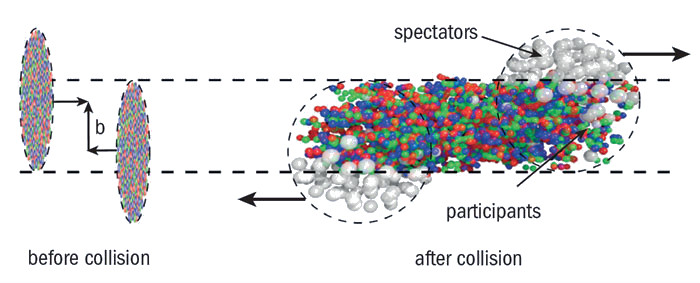
\includegraphics[scale=0.5]{introduction/figs/glauber.png}
    \caption{The basic picture of a heavy-ion collision \cite{participants}. Nucleons that experience a collision are called participants, while those that do not are called spectators. These spectators are assumed to fly off in a straight path. Nucleons that suffer an inelastic collision are called wounded nucleons.}
    \label{fig:spectators}
\end{figure}


\subsubsection{QGP Signatures \& Small Systems}
There are many signatures of QGP formation in heavy-ion collisions, including, but not limited to:

\begin{enumerate}
    \item Jet Quenching: partons that eventually form the hadrons of a jet experience collisional energy loss and radiative energy loss in the QGP, much like bremsstrahlung radiation. 
    \item Flow: the hydrodynamic flow in the QGP leads imprints itself in correlations of final-state particles. 
    \item Strangeness Enhancement: strange quark production increases relative to up and down quark production. 
\end{enumerate}

We mention these signatures because of their relevance to correlation analyses, the topic of this thesis. While QGP formation in Pb-Pb collisions was not a surprise, smaller systems such as p-Pb and p-p show collective effects and strangeness enhancement that indicate the creation of QGP droplets. In fact, p-p is often taken as a reference to Pb-Pb data, serving as a normalization that allows us to interpret results from heavy-ion collisions.  \cite{Florkowski:pheno}. In addition, p-Pb is utilized to disentangle cold nuclear matter effects. If a medium is indeed formed in these smaller systems, then it calls into question our understanding of the QGP. To date, jet quenching has not been observed in p-p or p-A collisions, and light-ion runs are needed to gauge the expected magnitude of jet quenching in small systems \cite{Achenbach:2023pba}. Determining whether a medium is created in small system, in essence, the limits of QGP formation, is the underlying motivation behind this thesis. 


\subsection{The Origins of Strangeness Enhancement}
The ordinary protons and neutrons that make up the baryonic matter we interact with contain only up and down valence quarks\footnote{We are ignoring a discussion of the quark sea.}. At the Large Hadron Colliders, we can access energies required to produce strange and anti-strange quarks. For a given hadron, the net strangeness is defined as:

\begin{equation}
    S = -(n_s - n_{\bar{s}})
\end{equation}

where $n_s$ is the number of strange quarks and $n_{\bar{s}}$ is the number of anti-strange quarks. Note that a strange quark has $S=-1$. The minus sign is an arbitrary choice to match the sign of the electric charge. To leading order, there are 4 diagrams that describe strangeness production. Since flavor is conserved, any strangeness we observe must orginate from an $s\bar{s}$ pair.\footnote{However, there must be some process that admits matter-antimatter asymmetry in the early universe, otherwise we wouldn't be here!} As suggested by Rafelski and M{\"u}ller in 1982, it turns out that enhanced strangness production in heavy-ion collisions could signify the creation of a QGP \cite{Rafelski:1982pu}. This occurs because gluon fusion (the top left diagram in Fig. \ref{fig:strange_diagram}) can occur faster than $q\bar{q}\rightarrow s\bar{s}$. 

\begin{figure}[h]
    \centering
    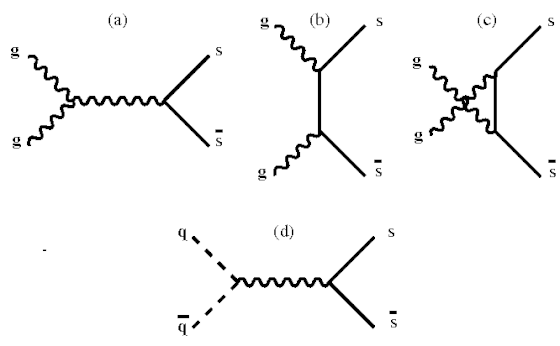
\includegraphics[scale=0.4]{introduction/figs/strangediagram.png}
    \caption{Leading order diagrams for strangeness production. Source: \textit{Wikipedia}.}
    \label{fig:strange_diagram}
\end{figure}

The enhancement of strangeness production can be quantified with the Wroblewski ratio:

\begin{equation}
    \lambda_s = \frac{2 \langle s\bar{s} \rangle}{\langle u\bar{u}\rangle + \langle d\bar{d}\rangle}
\end{equation}

Thus, we can calculate this ratio as a function of multiplicity (system or medium size). If we see an increase from "small systems" like p-p and p-Pb to Pb-Pb, we've found a signature of QGP formation. This strangeness enhancement has been observed and is shown in Fig. \ref{fig: s_enhacement}. Strangness enhancement seems to saturate as multiplicity increases. Interestingly, high multiplicity p-Pb collisions feature strangness enhancement that overlaps with low multiplicity Pb-Pb collisions. This suggests possible QGP formation in p-Pb, which is related to the idea of medium formation in small systems. Thus, by understanding the mechanism behind strangness enhancement in p-Pb, we can begin to determine whether we are creating a QGP in small systems. 


\begin{figure}[h]
    \centering
    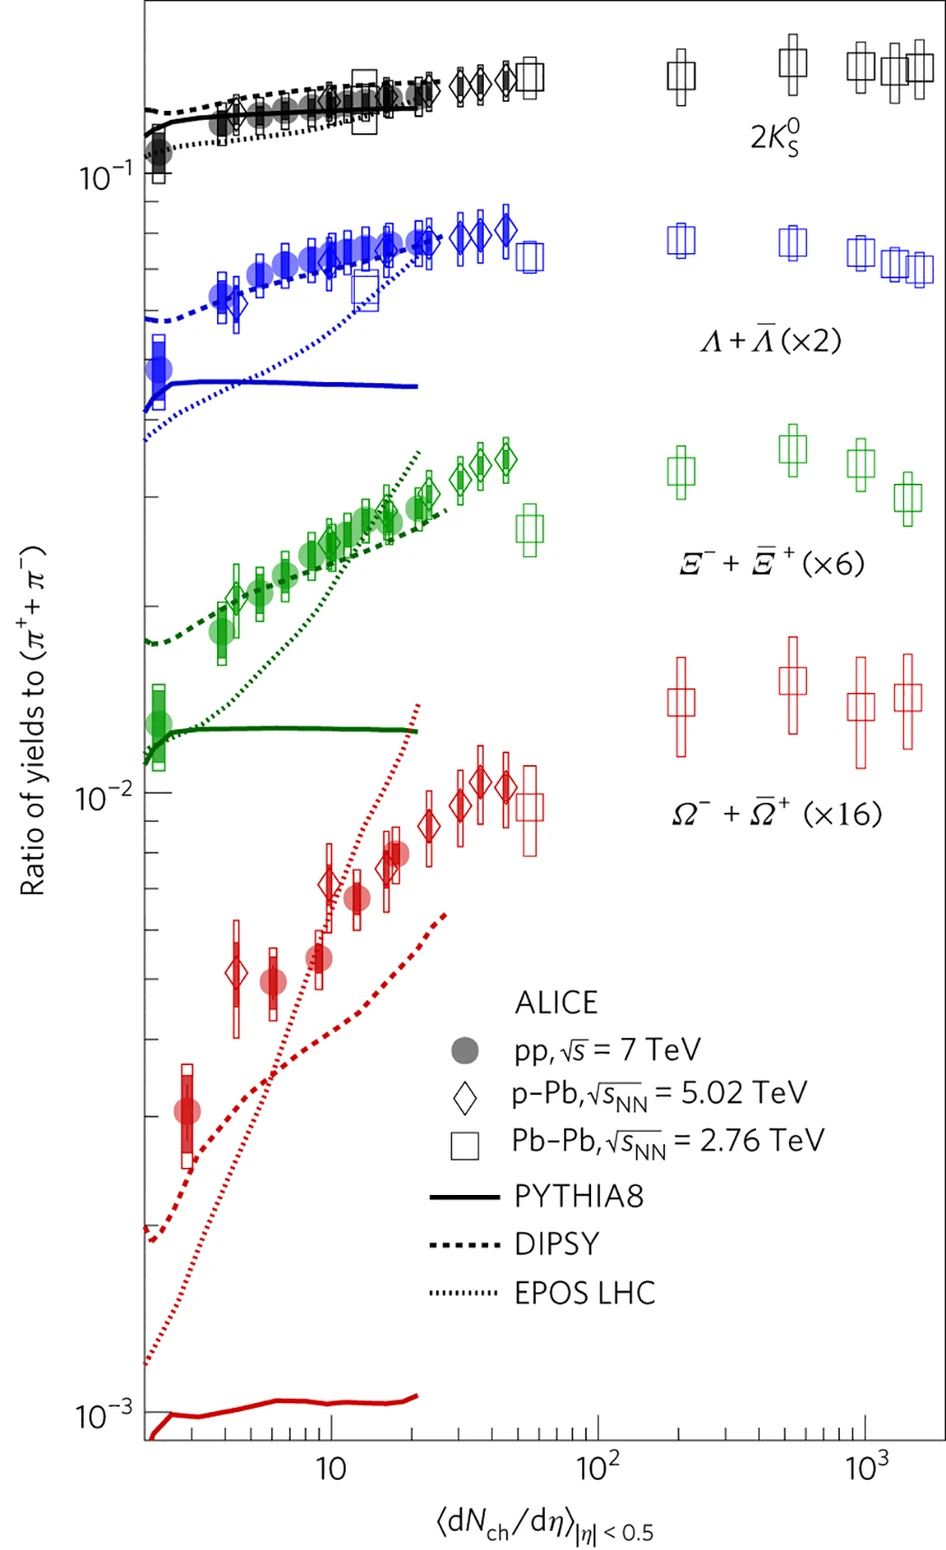
\includegraphics[scale=0.2]{strangeness_enhancement_1606_07424.png}    
    \caption{ALICE data demonstrating strangeness enhancement. The horizontal axis represents multiplicity.}
    \label{fig: s_enhacement}
\end{figure}

\clearpage
\section{A Large Ion Collider Experiment (ALICE)}
The Large Hadron Collider is the world's premier hadron collider, capable of accelerating protons and lead ions to near luminal speeds. This allows physicists to probe the interactions between fundamental particles, exploring the implications of the Standard Model and searching for new physics. The collision systems and energies\footnote{If you're curious why we use $\sqrt{s}$ for the center-of-mass energy, read up on Mandelstam variables.} at the LHC are: 

\begin{center}
    \begin{tabular}{|c|c|} 
        \hline
        System & Energy \\
        \hline
        Proton-Proton (p-p) & $\sqrt{s} = 13.6$ TeV \\ 
        %
        Proton-Lead (p-Pb) & $\sqrt{s_{NN}} = 8.16$ TeV \\
        %
        Lead-Lead (Pb-Pb) & $\sqrt{s_{NN}} = 5.36$ TeV \\
        \hline
    \end{tabular}
\end{center}

Note that these energies are tiny. The average housefly has a maximum speed of around $2.3$ m$\text{s}^{-1}$ and an average mass of $12$ mg. Thus, a fly has almost $14,000$ times the kinetic energy in a p-p collision. The key is the Large Hadron Collider is capable of creating systems with incredible energy density; individual protons are much smaller than a fly.  

At the LHC, there are two beamlines that cross at four \textit{interaction points}. These interaction points are the locations of the LHC's major experiments: ATLAS, ALICE, CMS, and LHCb. Each beamline carries bunches of protons or lead ions, that pass through each other at the interaction points---a bunch crossing. This produces the collisions we seek to untangle but also a background in the form of pile-up.

The ALICE experiment at the LHC is a dedicated experiment for relativistic heavy-ion physics, specializing in the identification and characterization of low-momentum particles. ALICE weighs approximately $10,000$ metric tons and has dimensions of $16\times16\times26$ $\text{m}^3$ \cite{ALICE:tdr}. By using various layers of detectors, ALICE obtains the kinematic information that becomes the backbone of analyses. At the heart of particle detection and measurement is the concept of a \textit{track}, a path a particle takes in the detector as it travels through the various components. For reasons given in Section \ref{section:tpc}, a large magnetic field is maintained in the inner barrel of the ALICE detector, causing charged particle to create curved tracks. Identifying these tracks is a challenge, especially with the high multiplicities of heavy-ion collisions, meaning a high track density. Tracing the path of a particle through multiple complicated detectors requires extraordinary synchronization of many components. Below, we touch on the basics of particle identification and measurement. 

\begin{figure}[h]
    \centering
    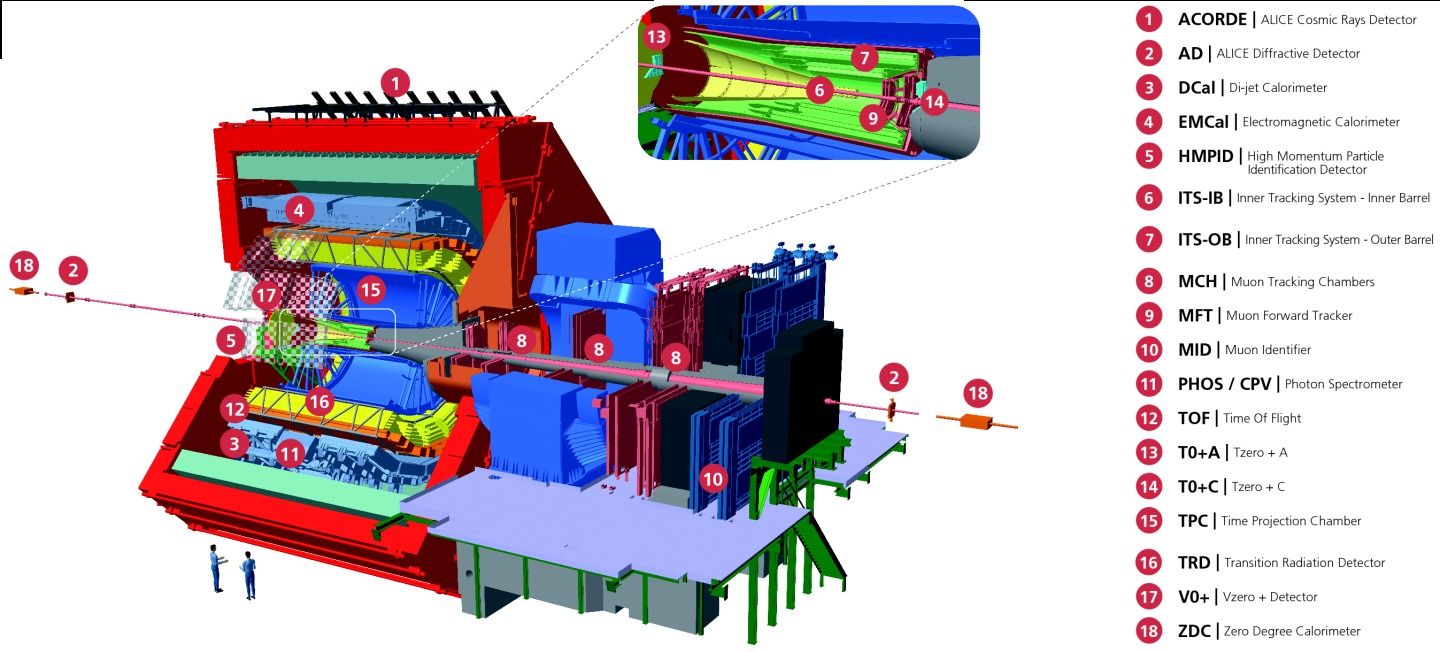
\includegraphics[scale=0.3]{alice_run3_schematic.jpeg}
    \caption{A schematic of the ALICE experiment during Run 3 \cite{ALICE:schematic}. The proceeding sections will follow the path a particle takes through the various detectors.}
    \label{fig:alice_schematic}
\end{figure}


Often, it is useful to define a \textit{separation power} that quantifies our ability to discriminate between two different types of particles. Given a detector resolution of $\sigma$, this separation power is given by \cite{Thomson:particle}:

\begin{equation}
    \label{eq:nsigma}
    n_\sigma = \frac{R_A - R_B}{\sigma}
\end{equation}

where $R_A$ is the average response of the detector to particle species $A$ and $R_B$ is the average response to particle species $B$. As $\sigma$ increases, the separation power decreases, corresponding to a poor ability to discriminate. A large difference in response enables a better ability to discriminate. To ensure the quality of tracks, one might exclude tracks with small $n_\sigma$.

\begin{figure}[h]
    \centering
    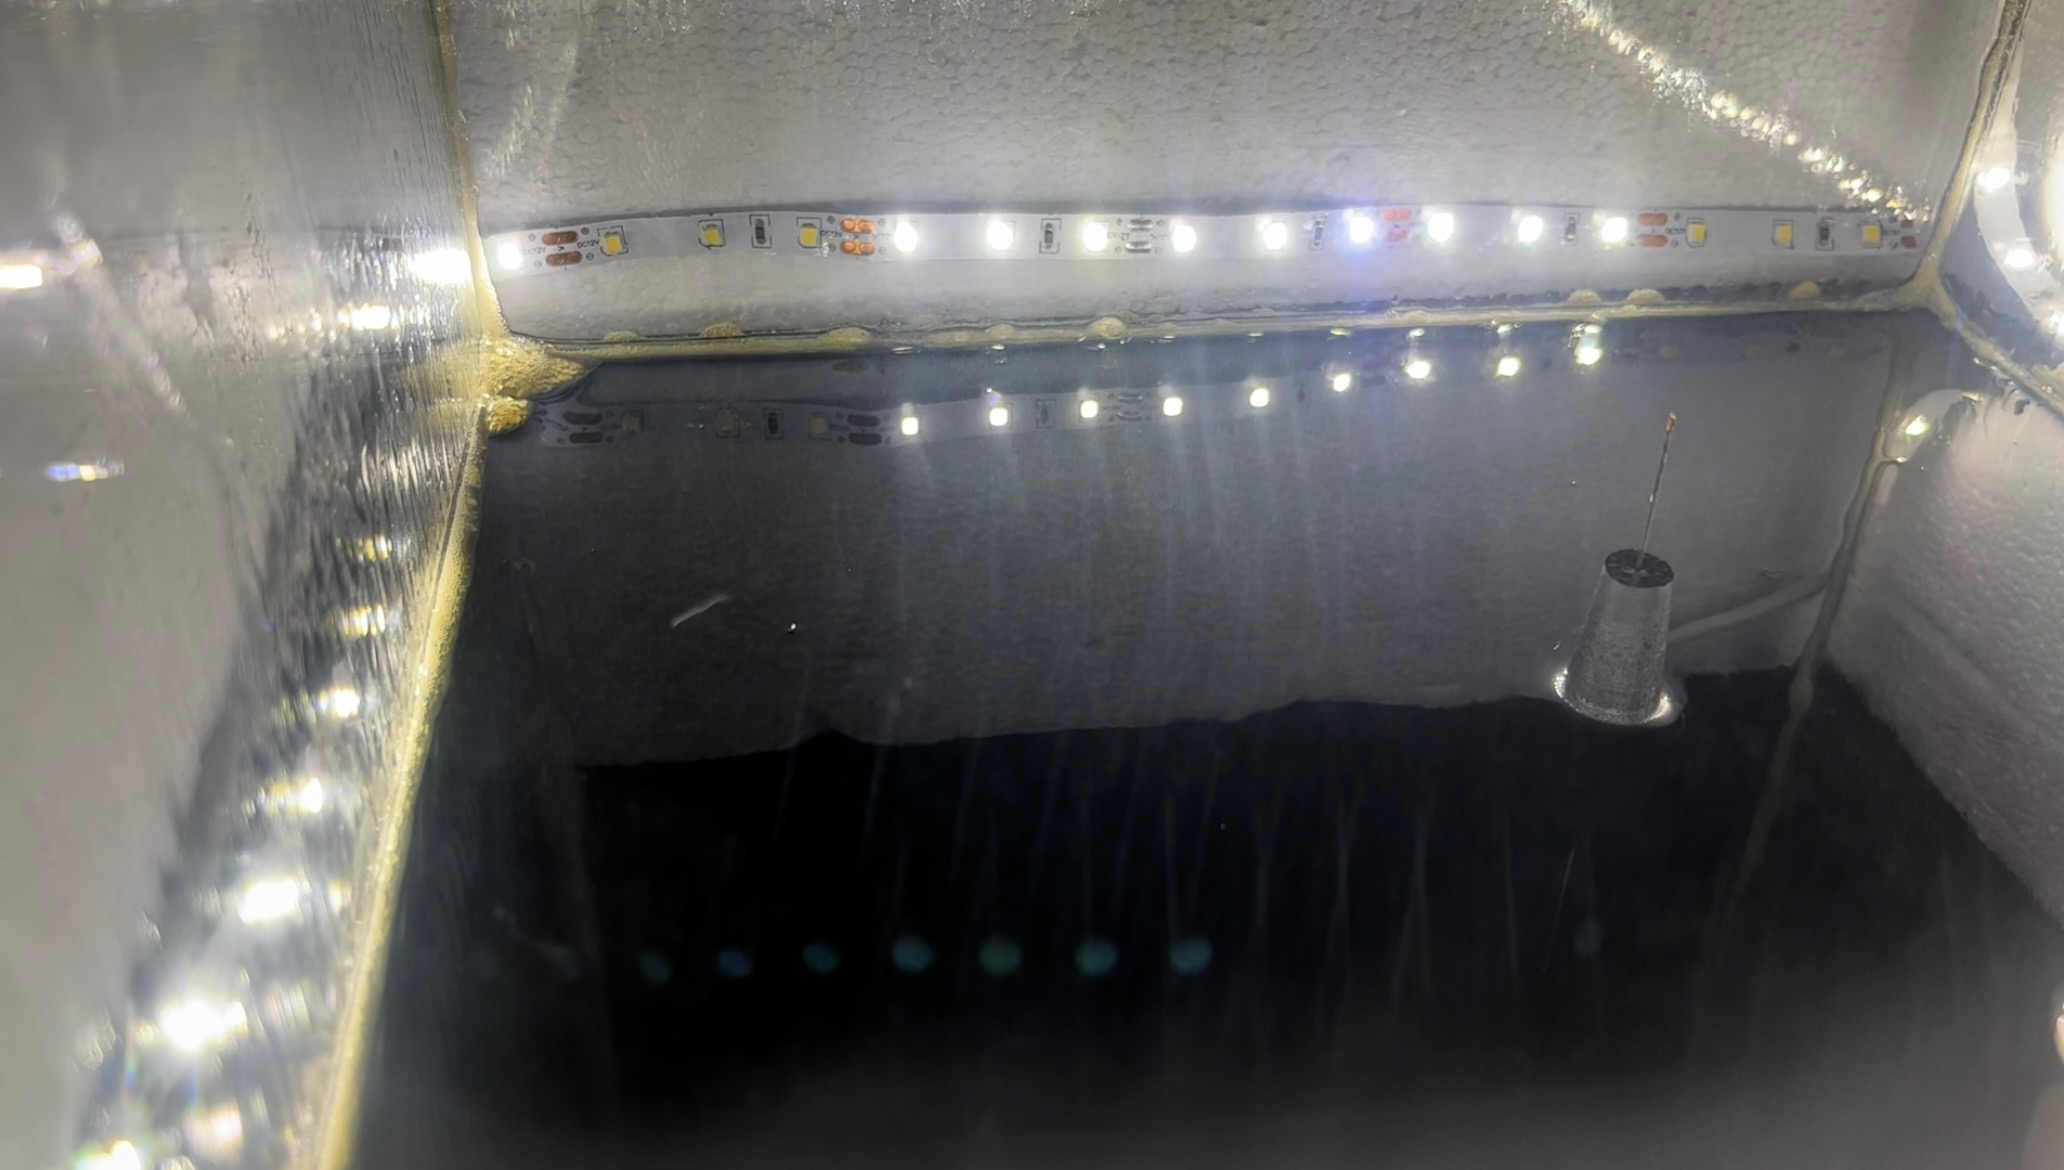
\includegraphics[scale=0.15]{introduction/figs/cloud.jpeg}
    \caption{A cloud chamber built by the author of this thesis and another University of Texas undergraduate. The small white streak towards the left of the photo is an alpha track, produced when a helium nucleus causes supersaturated alcohol at the bottom of the chamber to condense. The concept of a track has its roots in early cloud and bubble chambers used to unravel the particle zoo.}
    \label{fig:cloud}
\end{figure}


\subsection{Inner Tracking System (ITS)}
The inner tracking system (ITS) is the closest detector the beamline, consisting of $6$ layers of silicon detectors with an overall pseudorapidity coverage of $|\eta| \leq 0.9$ \cite{ALICE:tdr}. These silicon detectors are capable of dealing with high track density near the beamline, which is vital for heavy-ion collisions. In particular, the ITS is used to locate the primary vertex, the initial collision point, and secondary vertices, the location of weak decays that occur after the initial collision (eg. the decays of hyperons or B mesons). The $4$ outermost layers of the ITS read out an analog signal which is used for particle identification via the Bethe-Bloch equation for $dE/dx$, explained in the next section \cite{ALICE:tdr}. The innermost layers simply register hits. The ITS has good spatial resolution for particles and tracks. 

\begin{figure}[h]
    \centering
    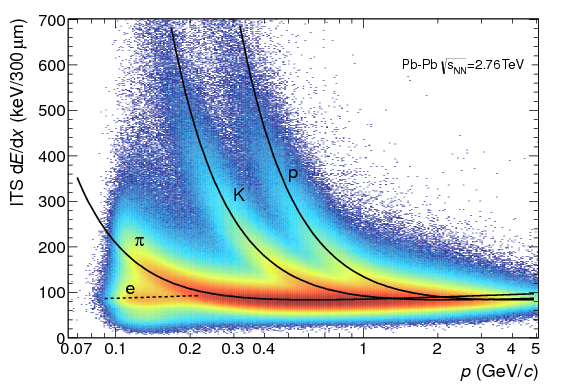
\includegraphics[scale=0.5]{its_dedx.png}
    \caption{$dE/dx$ curves of particles in the ITS. The ITS measures both $dE/dx$ and $p$ \cite{ALICE:performance}.}
    \label{fig:its_dedx}
\end{figure}

\subsection{Time Projection Chamber (TPC} \label{section:tpc}
The ALICE time projection chamber (TPC)\footnote{LUX-ZEPLIN, a WIMP dark matter direct detection experiment, is essentially one giant TPC. The author of this thesis worked on an ML algorithm for event identification in this TPC.} is a large volume filled with gas, used for particle identification and tracking with pseuodrapidity coverage of $|\eta|<0.9$. When a charged particle passes through, it ionizes the gas. The ionization electrons then drift along the $z$ axis due to an applied electric field and are measured when they reach the end-plates. A measurement of the drift time gives a location in $z$. Where the electron deposits on the end-plates gives the $x$-$y$ coordinates. This position information is used to reconstruct particle tracks in the detector.\footnote{Ordinary tracking, or 3D tracking, consists of points with 3 spatial coordinates. LHCb has suggested 4D tracking, where each point in a track also has an associated time \cite{LHCb:upgrades}.}  

An applied $\vec{B}$ field causes tracks to curve in a helix, giving us information about each particle's momenta. In the transverse plane, this motion is a circle, so from Newton's second law:

\begin{align}
    qvB &= m\frac{v_T^2}{R} \\ 
    qB &= \frac{mv_T}{R} \\
    qBR &= mv_T = p_T
\end{align}

where $q$ is the charge of the particle, $v_T$ is the transverse velocity, $B$ is the magnetic field strength, and $R$ is the radius of curvature. The final state particles that reach the TPC will have charge $\pm e$, meaning we can measure the momentum of a charged particle that makes a track in the TPC. The direction the track curves in gives the sign of the charge. 

\begin{figure}[h]
    \centering
    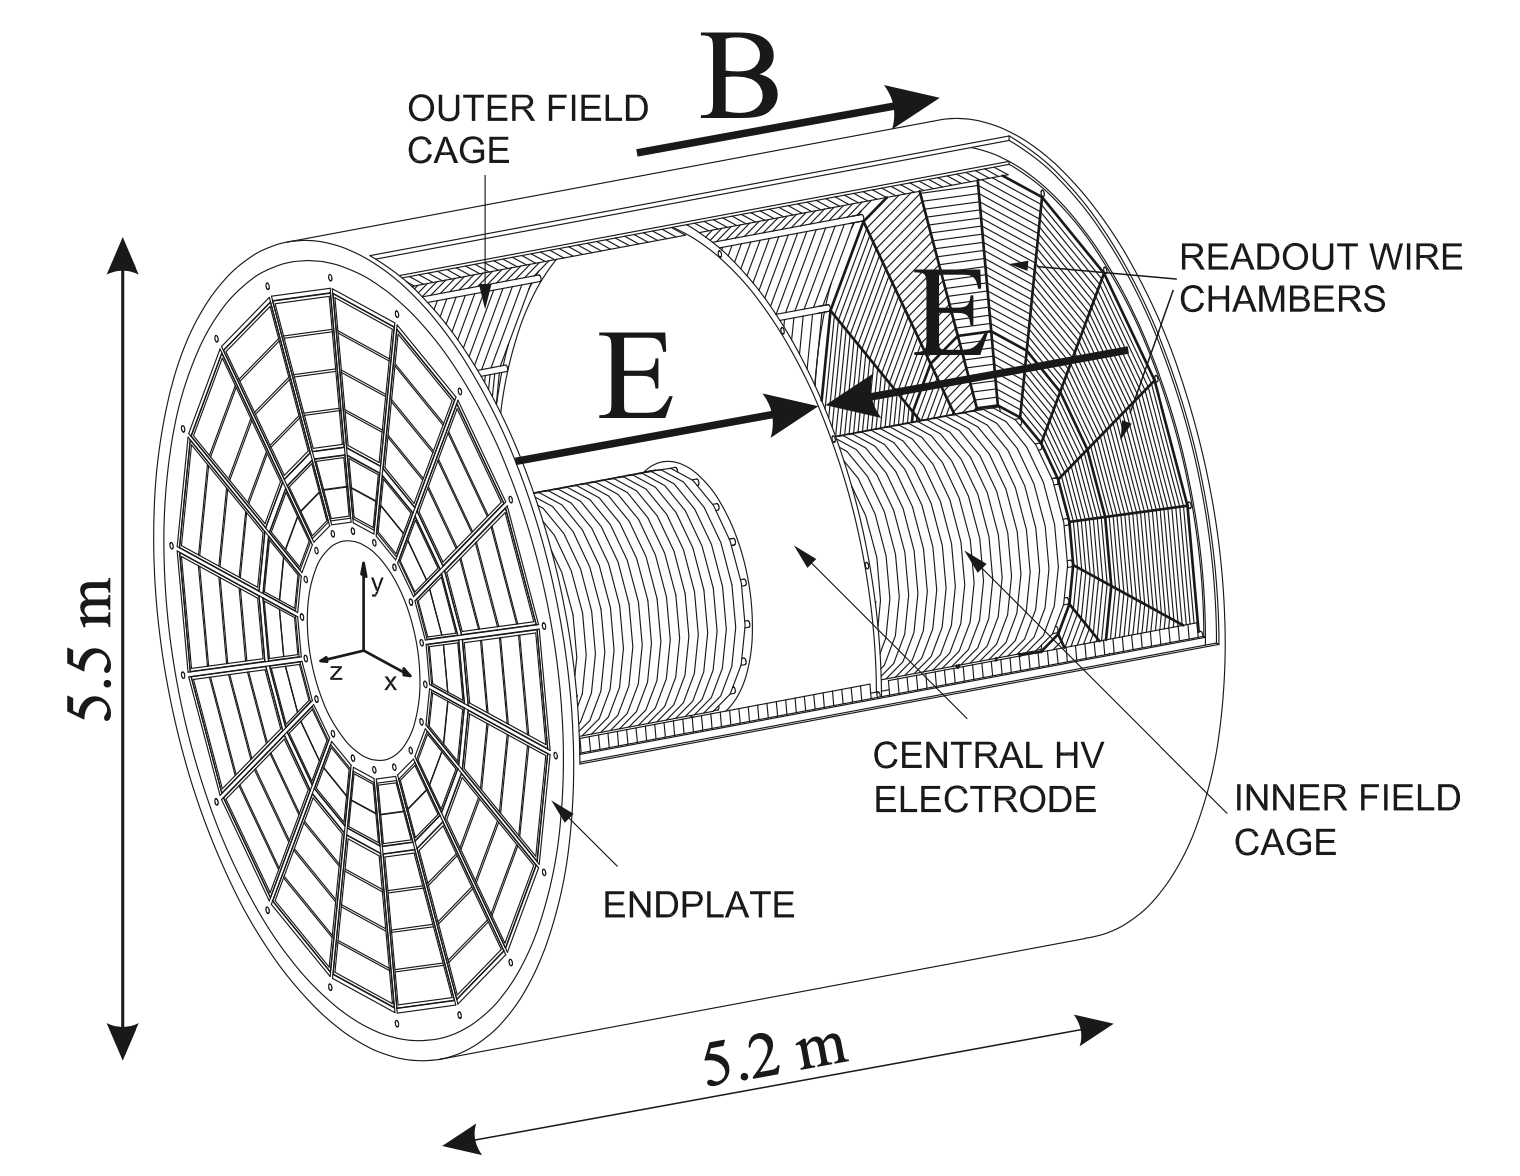
\includegraphics[scale=0.4]{alice_tpc_schematic.png}
    \caption{A schematic of the ALICE TPC, modified in \cite{detectors} and originally found in \cite{ALICE:tpc}}. Note that the TPC is large enough to stand in!
\end{figure}

Relativistic charged particles traveling through the TPC lose energy as they interact with the electrons of the gas molecules, inducing ionization of the gas \cite{Thomson:particle}. The mean rate of energy loss for a particle that travels through the medium is given by the Bethe-Bloch equation \cite{Bichsel:2004ej}:

\begin{equation}
    \left\langle -\frac{dE}{dx} \right\rangle = Kz^2\frac{Z}{A}\frac{1}{\beta^2}\left[\frac{1}{2}\ln\frac{2m_ec^2\beta^2\gamma^2W_{\text{max}}}{I^2}-\beta^2-\frac{\delta(\beta\gamma)}{2}\right]
\end{equation}

where $K \approx 0.307$ MeV $\text{cm}^2$ $\text{mol}^{-1}$ is a constant, $z$ is the charge of the particle in electron charges, $Z$ is the atomic number of the medium, $A$ is the atomic mass of the medium, $\beta$ is the speed of the particle over $c$, $m_e$ is the mass of an electron, $c$ is the speed of light, $\gamma$ is the Lorentz factor, $W_{\text{max}}$ is the maximum kinetic energy the particle can transfer to an electron in the medium in a given collision, $I$ is the mean excitation energy, and $\delta$ is a correction term. This gives the energy loss per distance travelled in the medium in terms of properties of the particle and its velocity. This energy loss is measured from the drift electrons collected at the end-plates.

In practice, ALICE utilizes a different parametrization of the Bethe-Bloch formula \cite{Yu:2013dca}:

\begin{equation}
    \label{eq:dedx}
    f(\beta \gamma) = \frac{P_1}{\beta^{P_4}} \left(P_2 - \beta^{P_4} -\ln\left(P_3 + \frac{1}{(\beta\gamma)^{P_5}}\right)\right)
\end{equation}

where $P_{1-5}$ are parameters determined by the gas mixture in the TPC. Since we can gather information about the particle's momentum from the TPC, this parametrization is commonly written in terms of the mass and momentum of the particle using:

\begin{equation}
    \label{eq:beta}
    \beta = \frac{\gamma m \beta}{\gamma m} = \frac{p}{E} = \frac{p}{\sqrt{m^2 + p^2}}
\end{equation}

where we assume natural units. Thus, if we plot $dE/dx$ against $p$, each particle will produce a different curve that depends on its mass (Fig. \ref{fig:dedx_tpc}). With these curves, we can perform particle identification with the TPC. Note that for large $p$, the curves begin to approach each other, making identification more challenging in this region. In Eq. \ref{eq:nsigma}, we introduced the idea of a separation power. For the TPC, we calculate a similar---but different---quantity using

\begin{equation}
    n_{\sigma, \text{TPC}} = \frac{dE/dx_{\text{meas}} - dE/dx_{\text{exp}}}{\sigma_{TPC}}
\end{equation}

where $dE/dx_{\text{meas}}$ is the measured rate of energy loss, $dE/dx_{\text{exp}}$ is the expected rate of energy loss for a given species (calculated from the fits shown in Fig. \ref{fig:dedx_tpc}), and $\sigma_{\text{TPC}}$ is the resolution of the TPC. 


\begin{figure}[h]
    \centering
    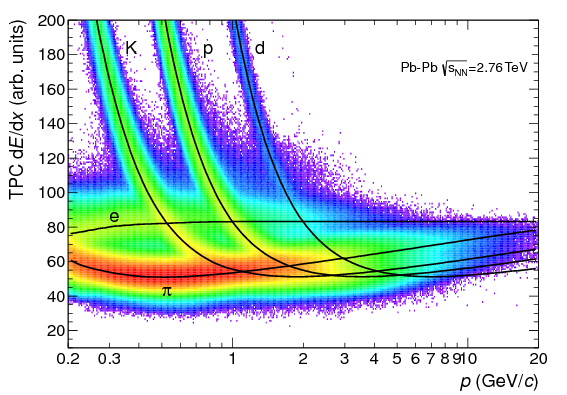
\includegraphics[scale=0.5]{tpc_dedx.png} 
    \caption{The rate of energy loss versus momentum in the TPC. The black lines corresponds to fits using Eq. \ref{eq:dedx}}
    \label{fig:dedx_tpc}
\end{figure}

\subsection{Time-of-Flight (TOF)}

The time-of-flight detector (TOF) is used for particle identification and triggers both cosmic ray events and ultraperipheral collisions \cite{Carnesecchi:2018oss}. The TOF is located $3.7$ m, just outside of the TPC, and covers $|\eta|<0.9$. By measuring the time between the initial interaction and when the particle reaches the TOF, we can reconstruct the particle's velocity. The start time for the TOF to begin the measurement is triggered by the T$0$ detector \cite{ALICE:performance}. If we let $d$ be the distance from the interaction point to the TOF and $\Delta t$ be the time between the interaction and when the particle reaches the TOF, then the velocity $v$ of the particle is given by:

\begin{equation}
    v = \frac{d}{\Delta t} = \frac{p}{\sqrt{m^2 + p^2}}
\end{equation}

where we use natural units. From Eq. \ref{eq:beta}, we can relate the velocity to the momentum of a particle. Since each particle has a distinct mass, each particle creates a unique band in a plot of $v$ versus $p$ (Fig. \ref{fig:tof_bands}). Additionally, as with the TPC, we can define:

\begin{equation}
    n_{\sigma, \text{TOF}} = \frac{\beta_{\text{meas}} - \beta_{\text{exp}}}{\sigma_{TOF}}
\end{equation}

where $\beta_{\text{meas}}$ is the measured velocity over $c$ in the TOF, $\beta_{\text{exp}}$ is the expected velocity over $c$, and $\sigma_{\text{TOF}}$ is the resolution of the TOF.


\begin{figure}[h]
    \centering
    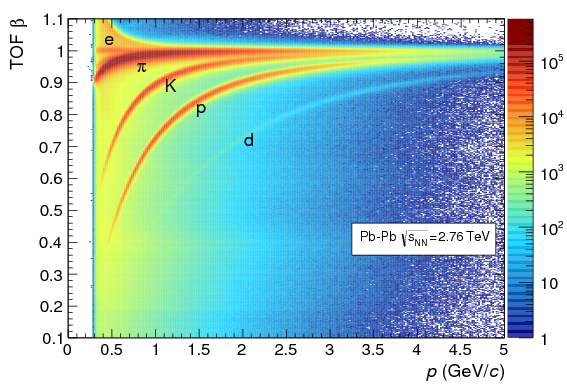
\includegraphics[scale=0.5]{tof_bands.png}
    \caption{$\beta$ versus $p$ curves from the TOF. Unphysical values of $\beta$ come from when hits are assigned to the wrong track \cite{Carnesecchi:2018oss}.}
    \label{fig:tof_bands}
\end{figure}

\subsection{Calorimetry}
While not necessary for our analysis, a discussion of general collider physics would be remiss without a mention of calorimetry. A \textit{calorimeter} is a detector that measures the energy deposition due to a particle. Some experiments like sPHENIX at the Relativistic Heavy-Ion Collider have both electromagnetic and hadronic calorimeters. In the case of ALICE, the main calorimeter is the Electromagnetic Calorimeter (EMCal), which is used to identify electrons and photons. The EMCal is also used to detect neutrons and $\pi^0$ decays. In particular, the EMCal is important for identifying heavy-flavor electrons that result from semileptonic decays (a weak decay in which a lepton, neutrino, and hadron are produced) \cite{ALICE:performance}.

High energy electrons moving through a medium produce bremsstrahlung (braking) radiation. If the bremsstrahlung photon has high enough energy, it can pair produce into an electron and positron, which in turn will produce more bremsstrahlung radiation which causes more pair production. This creates an \textit{electromagnetic shower} which continues until enough energy is lost for pair production to cease (Fig. \ref{fig:em_shower}).  An EMCal utilizes materials with large atomic number as scintillators. Electrons produced in an electromagnetic shower induce light via scintillation, which is measured in sensitive photon detectors \cite{Thomson:particle}. A charged track that enters the EMCal and produces an electromagnetic shower signifies an electron, while a photon might deposit energy in the EMCal without producing a shower. The ALICE EMCal can be used to trigger on events with a jet, by recording an event if the transverse energy in part of the EMCal rises above a certain threshold \cite{ALICE:performance}. In general, hadronic calorimetry is significantly harder because a variable, non-negligible fraction of the incoming hadron's energy goes into undetectable channels \cite{detectors}. Since ALICE specializes in the identification of low-momentum particles, a hadronic calorimeter is unnecessary. 

\begin{figure}[h]
    \centering
    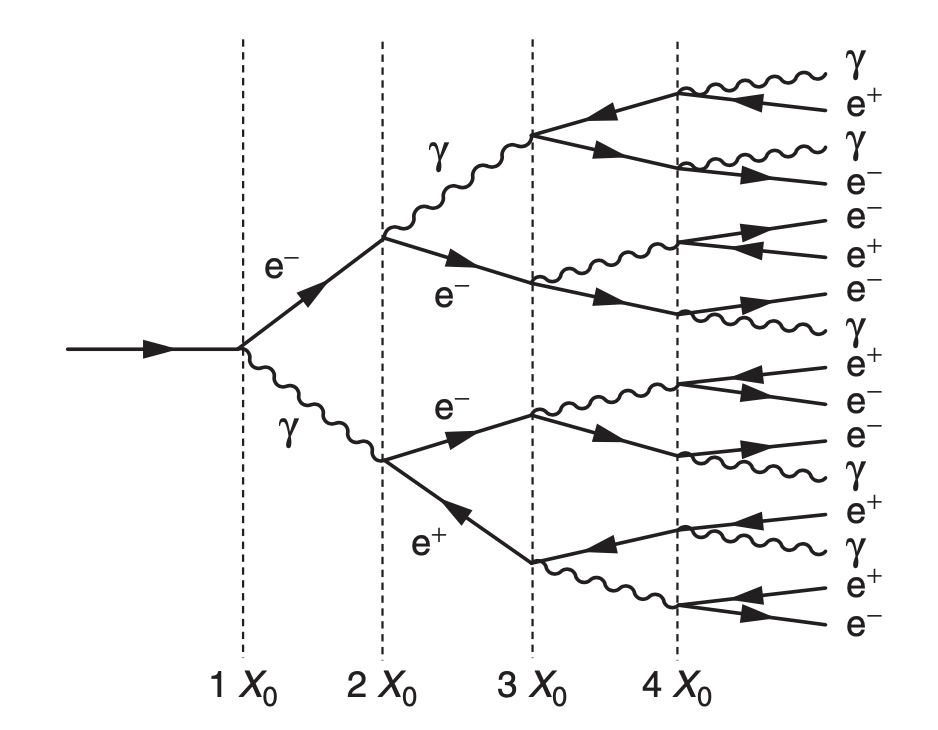
\includegraphics[scale=0.4]{emshower.png}
    \caption{A diagram of an electromagnetic shower \cite{Thomson:particle}. Here $X_0$ represents a characteristic radiation length after which the number of particles doubles.}
    \label{fig:em_shower}
\end{figure}


\begin{figure}[h]
    \centering
    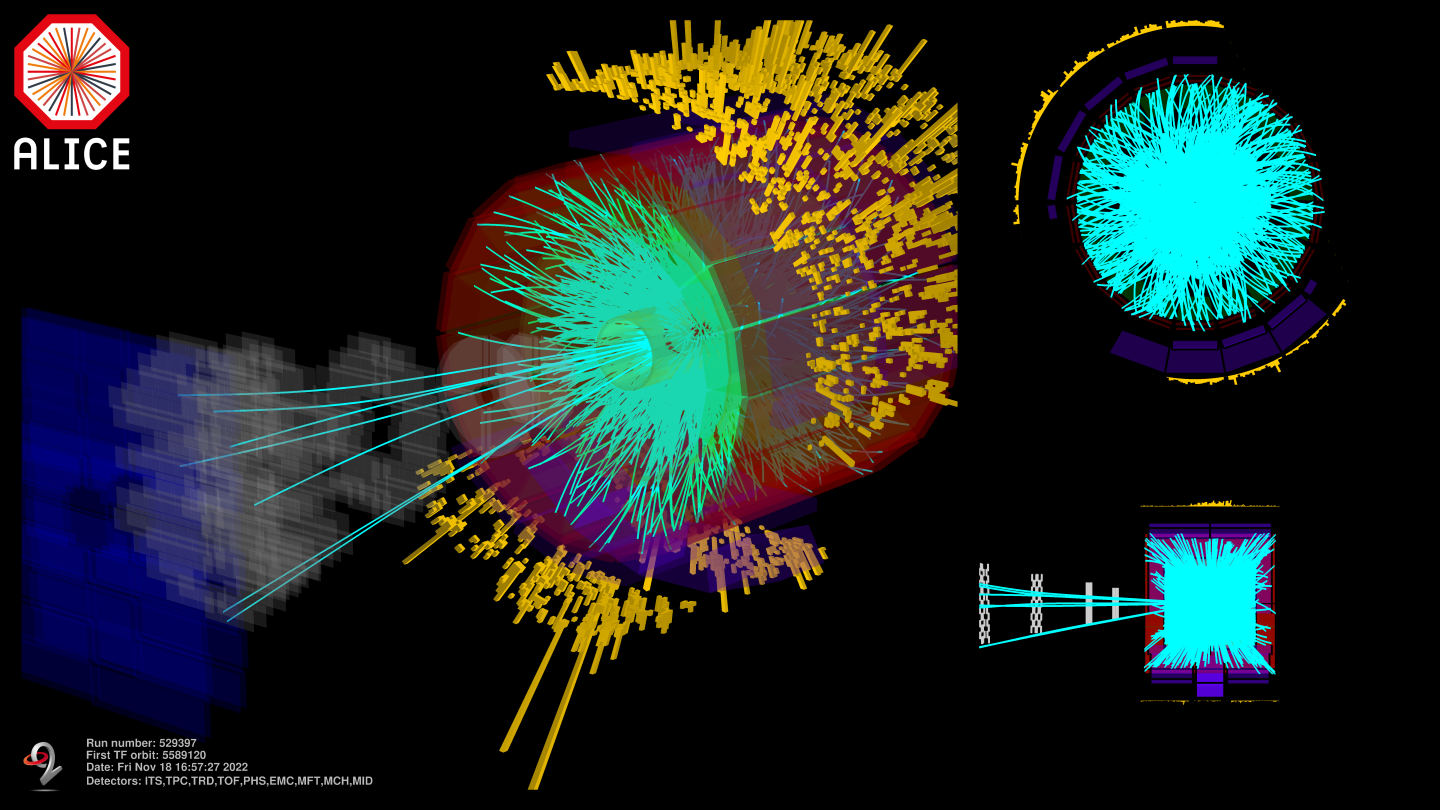
\includegraphics[scale=0.2]{2022_nov_18.png}
    \caption{Tracks in the ALICE experiment, along with depositions in the calorimeters. This event display is from the start of Run 3 after upgrades to ALICE, including the ITS. The author of this thesis was just starting in heavy-ion physics when these images were released!}
\end{figure}


\subsection{VZERO}
The VZERO system is composed of the VZERO-A and VZERO-C detectors, which are located in the forward regions at $2.8<\eta<5.1$ and $-3.7<\eta<-1.7$. These detectors are used to trigger events, reject beam-gas interactions, and measure event multiplicity \cite{ALICE:2013axi}. By measuring energy deposition, the VZERO system can determine the charged particle multiplicity of the event. This is critical in heavy-ion collisions because multiplicity tells us how central or peripheral a collision was.  

\begin{figure}[h]
    \centering
    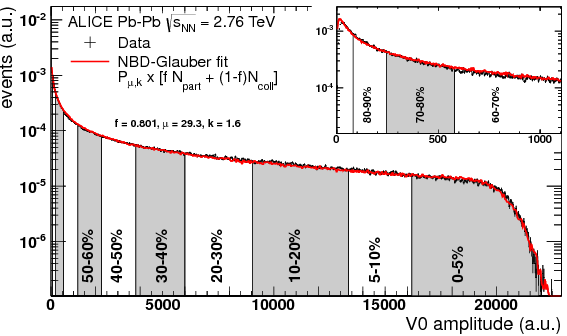
\includegraphics[scale=0.4]{VZERO_activity.png}
    \caption{The amplitude in the VZERO detector, separated into centrality classes. The Glauber fit refers to the Glauber model, which is used to understand heavy-ion collisions \cite{Florkowski:pheno}.}
\end{figure}


\ifSubfilesClassLoaded{%
    \printbibliography
}

\end{document}